%%%%%%%%%%%%%%%%%%%%%%%%%%%%%%%%%%%%%%%%%%%%%%%%%%%%%%%%%%%%
% PREÁMBULO — DOCUMENTO EJECUTIVO
%%%%%%%%%%%%%%%%%%%%%%%%%%%%%%%%%%%%%%%%%%%%%%%%%%%%%%%%%%%%

\documentclass[11pt,a4paper]{article}

% --- CODIFICACIÓN & IDIOMA ---
\usepackage[utf8]{inputenc}
\usepackage[T1]{fontenc}
\usepackage[spanish, es-tabla]{babel} % "Tabla" en lugar de "Cuadro"

% --- TIPOGRAFÍA & MICROTIPOGRAFÍA ---
\usepackage{lmodern}         % fuente vectorial (ligera y limpia)
\usepackage[protrusion=true,expansion=true]{microtype}

% --- MATEMÁTICAS ---
\usepackage{amsmath, amssymb}
\numberwithin{equation}{section}

% --- TABLAS PROFESIONALES ---
\usepackage{booktabs}
\usepackage{threeparttable}  % notas al pie en tablas
\usepackage{siunitx}         % alineación numérica
\sisetup{
  output-decimal-marker = {,}, % convención española
  table-number-alignment = center,
  table-figures-integer = 3,
  table-figures-decimal = 2
}

% --- FIGURAS & GRÁFICOS ---
\usepackage{graphicx}
\graphicspath{{figures/}}    % carpeta de figuras
\usepackage[font=small,labelfont=bf,labelsep=period]{caption} % pies compactos
\usepackage{subcaption}      % subfiguras si las necesitas
\usepackage{placeins}        % \FloatBarrier para controlar flotantes

% --- COLOR & CAJAS EJECUTIVAS ---
\usepackage{xcolor}
\definecolor{brandblue}{HTML}{0D3B66}
\definecolor{brandorange}{HTML}{F4A261}
\usepackage[most]{tcolorbox}
\tcbset{
  sharp corners, colback=white, colframe=brandblue!60,
  left=6pt,right=6pt,top=6pt,bottom=6pt
}
\newenvironment{mensajeclave}{%
  \begin{tcolorbox}\bfseries Mensaje clave.\ }{\end{tcolorbox}}

% --- LISTAS COMPACTAS ---
\usepackage{enumitem}
\setlist{nosep,leftmargin=*,itemsep=1pt,topsep=3pt}

% --- HIPERVÍNCULOS & REFERENCIAS ---
\usepackage{hyperref} % (carga correcta; dejar esta)
\hypersetup{
  colorlinks=true,
  linkcolor=brandblue,
  citecolor=brandblue,
  urlcolor=brandblue,
  pdfauthor={Manuel Alejandro Hidalgo Pérez, Ernesto Talvi},
  pdftitle={Resumen Ejecutivo: Indicador de Vulnerabilidad Externa para Brasil}
}
\usepackage[nameinlink,capitalise,noabbrev]{cleveref} % después de hyperref

% --- CITADO APA ---
\usepackage{csquotes}
\usepackage[style=apa,backend=biber]{biblatex}
\DeclareLanguageMapping{spanish}{spanish-apa} % comentar si da error
\addbibresource{references.bib}

% --- MÁRGENES & PÁRRAFOS ---
\usepackage[left=2.5cm, right=2.5cm, top=3cm, bottom=3cm]{geometry}
\usepackage{parskip} % separación entre párrafos, sin sangría

% --- COMANDOS ÚTILES ---
\newcommand{\vect}[1]{\boldsymbol{#1}}
\DeclareMathOperator{\Var}{Var}
\DeclareMathOperator{\Cov}{Cov}

% --- TÍTULO ---
\title{
  \vspace{1cm}
  \LARGE{\textbf{Indicador de Vulnerabilidad Externa para Brasil}}\\
  \large{Una Herramienta Predictiva para la Toma de Decisiones}\\[0.5cm]
  \normalsize{Resumen Ejecutivo del trabajo de M.\ A.\ Hidalgo Pérez y E.\ Talvi}
}

\author{
  Manuel Alejandro Hidalgo Pérez\thanks{Universidad Pablo de Olavide y Real Instituto Elcano. Email: \texttt{mahidper@upo.es}} 
  \and 
  Ernesto Talvi\thanks{Real Instituto Elcano. Email: \texttt{etalvi@rielcano.org}}
}

\date{\today} % o \date{Octubre de 2025}

\begin{document}
\maketitle
\thispagestyle{empty}

\begin{abstract}
\noindent
Este documento presenta un indicador de vulnerabilidad externa para economías latinoamericanas exportadoras de materias primas, con Brasil como caso de estudio. A diferencia de los índices compuestos tradicionales, nuestra metodología se basa en un modelo vectorial de corrección de errores (VECM) que transforma el marco retrospectivo de cointegración de Izquierdo et al.\ (2008) en una herramienta prospectiva de alerta temprana. El indicador integra dos componentes: el desequilibrio estructural respecto al equilibrio de largo plazo, medido por el término de corrección de error y su velocidad de ajuste; y el riesgo del entorno externo, capturado mediante funciones impulso-respuesta y matrices de covarianza condicional de shocks. Al ser completamente \emph{model-implied}, garantiza objetividad, trazabilidad y comparabilidad temporal. La validación empírica (2000--2024) confirma su capacidad predictiva: valores elevados del indicador anticipan sistemáticamente desaceleraciones del PIB a 1--2 trimestres, con una correlación de $-0.22$ (excluyendo COVID). Esta métrica ofrece una plataforma operativa para la gestión proactiva de riesgos macroeconómicos en la región.
\end{abstract}

\vspace{0.5cm}

\noindent\textbf{Palabras clave:} vulnerabilidad externa, VECM, cointegración, alerta temprana, América Latina, Brasil

\clearpage



% --- SECCIÓN 1 (VERSIÓN REVISADA) ---
\section{El Desafío: Anticipar la Vulnerabilidad Externa}

\paragraph{Motivación.}
Este resumen ejecutivo aborda el problema de \textbf{anticipar vulnerabilidad externa} en economías abiertas donde los \emph{términos de intercambio} y las \emph{condiciones financieras globales} condicionan el crecimiento. El indicador está diseñado para: (i) monitoreo macro-financiero periódico, (ii) apoyo a discusiones de política y (iii) señalización temprana de riesgos de crecimiento a 1--2 trimestres.

Las economías latinoamericanas exportadoras de materias primas enfrentan una exposición estructural a la volatilidad del entorno económico global. Las fluctuaciones en los precios de sus commodities, los cambios en las condiciones financieras internacionales, las variaciones en la demanda de sus socios comerciales y los movimientos en los flujos de capital pueden generar shocks externos de magnitud considerable. Estos eventos tienen profundas repercusiones sobre el crecimiento económico, la estabilidad macroeconómica y la sostenibilidad fiscal de la región. En este contexto, el desarrollo de herramientas robustas y oportunas para el monitoreo y la predicción de episodios de vulnerabilidad externa constituye una prioridad fundamental para la formulación de políticas efectivas y la gestión proactiva del riesgo sistémico.

Un sistema de alerta temprana eficaz, sin embargo, debe ir más allá de una simple señal de alarma. Para que sea verdaderamente útil para los responsables de política económica, debe ofrecer respuestas claras a una secuencia de preguntas críticas. Primero, es fundamental saber qué tanta presión contractiva sugiere el estado actual de la economía: dado el desvío acumulado respecto al equilibrio externo sostenible y la velocidad con la que tiende a corregirse, ¿cuál es el empuje previsto sobre el crecimiento a corto plazo? Segundo, esta medida de presión debe ser contextualizada por el nivel de incertidumbre vigente; un mismo impulso contractivo es más o menos preocupante según la volatilidad y las correlaciones recientes de los shocks externos relevantes. Finalmente, para que la métrica sea accionable y permita diseñar políticas correctivas, debe ser transparente. Es crucial poder identificar qué canal está detrás de cada episodio de vulnerabilidad, atribuyendo los cambios del indicador a variables específicas---como los términos de intercambio o las tasas globales---y evitando así los índices opacos basados en ponderaciones discrecionales.

% --- SECCIÓN 2 ---
% --- SECCIÓN 2 (VERSIÓN EXPANDIDA) ---
\section{La Anatomía del Indicador: del VECM a una señal en unidades de riesgo}

\subsection{Punto de partida: el marco de Izquierdo et al.}

Nuestra estrategia metodológica parte del influyente trabajo de \textcite{izquierdo2008booms}, quienes desarrollaron un marco empírico para identificar episodios de "paradas súbitas" (\emph{sudden stops}) y analizar sus determinantes macroeconómicos en economías emergentes. Su enfoque se basa en la estimación de relaciones de equilibrio de largo plazo entre variables clave—como el producto, los términos de intercambio y las condiciones financieras globales—mediante técnicas de cointegración. Este marco permite distinguir desviaciones cíclicas respecto a trayectorias sostenibles y vincular dichas desviaciones con episodios de crisis.

Sin embargo, el análisis de Izquierdo et al.\ es fundamentalmente \textit{retrospectivo}. Su objetivo principal consiste en caracterizar y explicar episodios de estrés ya ocurridos, identificando los factores que los precedieron. Para los fines de este trabajo—construir una herramienta de \textbf{alerta temprana} operativa para decisores de política—necesitamos dar un paso adicional: transformar este marco descriptivo en un \textbf{indicador prospectivo} que (i) cuantifique la vulnerabilidad contemporánea en una métrica única y comparable, (ii) ofrezca señales interpretables en tiempo real, y (iii) sea completamente trazable en sus componentes.

\subsection{De la cointegración a la vulnerabilidad: tres ingredientes clave}

La extensión que proponemos conserva la intuición económica del enfoque de cointegración—capturar el equilibrio externo sostenible y medir desvíos respecto a él—pero la reorienta hacia la construcción de un índice sintético con poder predictivo. Esta transformación requiere integrar tres elementos conceptuales que, si bien están implícitos en modelos de corrección de errores estándar, aquí se hacen explícitos y operativos:

\paragraph{1. Desequilibrio como \textit{presión de ajuste}.}
El término de corrección de error ($ECT_t$) mide cuánto se desvía el PIB de su nivel de equilibrio de largo plazo, dados los fundamentales externos (términos de intercambio, tasas de interés globales). En el enfoque tradicional, este desvío es un diagnóstico \textit{ex post}; aquí lo convertimos en una medida de \textit{presión de ajuste} multiplicándolo por su coeficiente de velocidad ($\alpha_y$). Esto nos dice no sólo "dónde estamos respecto al equilibrio", sino "qué tan fuerte es el empuje que ejerce ese desequilibrio sobre el crecimiento futuro".

\paragraph{2. Riesgo como \textit{contexto de incertidumbre}.}
Un mismo nivel de desequilibrio no tiene las mismas implicaciones en todo momento. Si el entorno global es estable, la corrección puede ser gradual y ordenada; si es volátil y los shocks externos están sincronizados, el ajuste puede ser abrupto y costoso. Por ello, incorporamos explícitamente una medida de \textbf{riesgo externo} ($\sigma_t$) que combina dos dimensiones: la \textit{sensibilidad} de la economía a distintos shocks (capturada por las funciones impulso-respuesta del modelo) y la \textit{volatilidad y covarianza} de esos shocks (estimada en ventanas móviles). Esta métrica nos permite ponderar la señal de desequilibrio por el nivel de incertidumbre vigente.

\paragraph{3. Normalización en $''$unidades de riesgo$''$.}
Finalmente, integramos desequilibrio y riesgo en una sola métrica comparable en el tiempo. La idea es expresar la presión contractiva en \textit{unidades estandarizadas de riesgo}, de modo que valores altos del indicador reflejen tanto un desequilibrio significativo como un entorno externo adverso. Además, introducimos un amplificador que incrementa el peso de la señal cuando la incertidumbre es extrema, reconociendo que en esos contextos incluso desequilibrios moderados pueden desencadenar ajustes severos.

\subsection{Implementación empírica: del modelo a la señal}

\paragraph{Paso 1: Estimación del VECM y diagnóstico de cointegración.}
Partimos estimando un modelo vectorial de corrección de errores (VECM) para Brasil sobre una muestra trimestral (2000T1--2024T4). El modelo tiene la siguiente estructura general:

$$
\Delta \vect{y}_t = \vect{\alpha}\,\vect{\beta}^{\top}\vect{y}_{t-1} + \sum_{i=1}^{p-1}\vect{\Gamma}_i\,\Delta\vect{y}_{t-i} + \vect{\Phi}\,\vect{x}_t + \vect{\mu} + \vect{\varepsilon}_t,
$$

\noindent donde $\vect{y}_t = (\log PIB_t,\, \log ToT_t,\, US10Y_t)^{\top}$ es el vector de variables integradas de orden uno, $I(1)$: $\log PIB_t$ (producto interior bruto real de Brasil), $\log ToT_t$ (términos de intercambio) y $US10Y_t$ (rendimiento del bono del Tesoro de EE.\,UU. a 10 años). El término $\vect{\beta}$ es el vector de cointegración ($r=1$) que define la relación de equilibrio de largo plazo, $\vect{\alpha}$ es el vector de coeficientes de ajuste (donde $\alpha_y < 0$ garantiza convergencia), $ECT_{t-1} = \vect{\beta}^{\top}\vect{y}_{t-1}$ es el término de corrección de error, $\vect{\Gamma}_i$ son las matrices de coeficientes de corto plazo para los rezagos $i=1,\ldots,p-1$, y $\vect{\varepsilon}_t$ es el vector de innovaciones con $\mathbb{E}[\vect{\varepsilon}_t]=\vect{0}$ y $\Var[\vect{\varepsilon}_t]=\vect{\Sigma}$.

Adicionalmente, incorporamos dos controles estacionarios $I(0)$ en niveles como variables exógenas: $\vect{x}_t = (\log IP^{G7}_t,\, Spread_t)^{\top}$, donde $\log IP^{G7}_t$ es la producción industrial ponderada del G7 (proxy del ciclo económico global) y $Spread_t$ es un \emph{spread} de riesgo soberano/emergente. El término $\vect{\Phi}$ representa la matriz de coeficientes asociados a estas exógenas, y $\vect{\mu}$ es el vector de constantes.

La especificación del VECM incluye una constante en la relación de cointegración y un número de rezagos $p$ seleccionado mediante criterios de información (AIC/BIC). Para el período de COVID-19, se introducen dummies acotadas que capturan el colapso y la recuperación sin contaminar la dinámica estructural del modelo. Las pruebas de Johansen sobre el bloque $I(1)$ indican la existencia de $r=1$ relación de cointegración (véase \cref{tab:stationarity_johansen}), y el coeficiente de ajuste del PIB cumple la condición $\alpha_y<0$, garantizando que los desvíos respecto al equilibrio se corrigen endógenamente en el tiempo.

\paragraph{Paso 2: Extracción de componentes del modelo.}
Del VECM estimado obtenemos tres ingredientes fundamentales:
\begin{itemize}[nosep]
  \item El \textbf{término de corrección de error} ($ECT_t$) y su dinámica de ajuste ($\alpha_y$), que juntos determinan la presión de desequilibrio $\mu_t = \alpha_y \cdot ECT_{t-1}$.
  
  \item Las \textbf{funciones impulso-respuesta} (IRFs) del PIB a shocks externos. A partir de la representación de media móvil (VMA) del VECM:
  $$
  \vect{y}_t = \vect{\mu} + \sum_{j=0}^{\infty}\vect{\Psi}_j\,\vect{\varepsilon}_{t-j},
  $$
  donde $\vect{\Psi}_j$ son las matrices de multiplicadores dinámicos obtenidas recursivamente desde los coeficientes estimados $\{\vect{\alpha}, \vect{\beta}, \vect{\Gamma}_i, \vect{\Phi}\}$. Las IRFs del PIB a un shock en la variable $k$ al horizonte $h$ están dadas por el elemento $(1,k)$ de la matriz $\vect{\Psi}_h$. 
  
  Consideramos cuatro shocks externos relevantes: términos de intercambio ($\Delta \log ToT_t$), tasas globales ($\Delta US10Y_t$), ciclo G7 ($\Delta \log IP^{G7}_t$) y \emph{spread} de riesgo ($\Delta Spread_t$). Para cada shock $k$, calculamos la respuesta acumulada del PIB a un horizonte operativo $H$ (típicamente 4 trimestres):
  $$
  g_k = \sum_{h=0}^{H} \text{IRF}_{PIB \leftarrow shock_k}(h) = \sum_{h=0}^{H} [\vect{\Psi}_h]_{1,k}.
  $$
  
  El \textbf{vector de sensibilidades} $\vect{g} = (g_1, g_2, g_3, g_4)^{\top}$ recoge así el impacto acumulado de cada shock sobre el PIB durante el horizonte de interés. Estas sensibilidades son completamente \textit{model-implied}: derivan directamente de la estructura dinámica estimada del VECM y capturan tanto los efectos contemporáneos como la propagación intertemporal de cada shock a través de los mecanismos de ajuste de corto y largo plazo del modelo.
  
  \item Las \textbf{innovaciones estructurales} del modelo, $\{\vect{\varepsilon}_t\}_{t=1}^{T}$, obtenidas como los residuos de la estimación del VECM. A partir de estas innovaciones estimamos, en ventana móvil de longitud $W$ (típicamente 40 trimestres), la matriz de covarianzas condicional:
  $$
  \Sigma_t = \frac{1}{W}\sum_{\tau=t-W+1}^{t}\vect{\varepsilon}_{\tau}\vect{\varepsilon}_{\tau}^{\top}.
  $$
  Esta matriz captura tanto la volatilidad individual de cada shock como su grado de sincronización (covarianzas entre shocks), permitiendo que $\Sigma_t$ evolucione en el tiempo y refleje cambios en el entorno de riesgo externo.
\end{itemize}

\paragraph{Paso 3: Construcción del índice sintético.}
Con estos elementos, construimos el indicador en dos etapas. Primero, medimos el \textit{desequilibrio} como el empuje de corto plazo que el equilibrio ejerce sobre la actividad:
$$
\mu_t = \alpha_y \, ECT_{t-1}.
$$
Cuando la economía está por encima del equilibrio de largo plazo, $ECT>0$ y, dado que $\alpha_y<0$, la presión es contractiva (más negativa $\mu_t$); si está por debajo del equilibrio, ocurre lo contrario y hay margen para recuperación.

Segundo, caracterizamos el \textit{riesgo} del entorno externo con una medida que combina sensibilidad y volatilidad:
$$
\sigma_t = \sqrt{\,\vect{g}^{\top}\, \Sigma_t \,\vect{g}\,}.
$$
Esta formulación tiene una interpretación intuitiva: $\sigma_t$ aumenta no sólo cuando cada shock individual es más volátil, sino también—y esto es crucial—cuando los shocks tienden a ocurrir de forma sincronizada, elevando el riesgo sistémico.

Finalmente, ambas piezas se integran en una métrica legible en "unidades de riesgo". Ésta es la única ecuación necesaria en el cuerpo del informe para entender el indicador final:
$$
V_t = \Big(-\,\frac{\mu_t}{\sigma_t}\Big)\times\Big(\frac{\sigma_t}{\sigma_{\text{ref}}}\Big)^{\lambda}.
$$
El primer término normaliza el empuje contractivo por el riesgo vigente, midiendo así el desequilibrio en "unidades estandarizadas" de riesgo. El segundo término actúa como un amplificador no lineal que otorga mayor peso a la señal en episodios de incertidumbre extrema—cuando el riesgo en sí mismo se convierte en el factor dominante—con sensibilidad controlada por el parámetro $\lambda$ y una escala de referencia $\sigma_{\text{ref}}$ (típicamente la mediana histórica) que asegura comparabilidad temporal. En la práctica, valores más altos de $V_t$ indican mayor vulnerabilidad contemporánea y se interpretan con los umbrales empíricos (percentiles 75 y 90) reportados en las figuras de resultados.

\subsection{Ventajas de este enfoque frente a índices compuestos tradicionales}

A diferencia de los índices de vulnerabilidad construidos mediante ponderaciones ad hoc o análisis de componentes principales, nuestro indicador es \textbf{\textit{model-implied}}: cada peso, cada sensibilidad y cada medida de riesgo deriva directamente de los parámetros estimados del VECM. Esto garantiza tres propiedades deseables:

\begin{enumerate}[nosep]
  \item \textbf{Objetividad}: No hay decisiones discrecionales sobre qué pesos asignar a cada variable. Los pesos son los que el modelo identifica como óptimos dada la estructura de los datos.
  \item \textbf{Trazabilidad}: Cada observación del indicador puede descomponerse para diagnosticar qué está detrás de la señal: si domina el desequilibrio estructural (términos de intercambio deteriorados, por ejemplo) o si domina el riesgo externo (endurecimiento financiero global, mayor sincronización de shocks).
  \item \textbf{Coherencia temporal}: Al estar anclado en una relación de equilibrio de largo plazo, el indicador es comparable en distintos períodos, facilitando la interpretación de niveles absolutos y no solo de cambios relativos.
\end{enumerate}

En resumen, esta sección ha expuesto cómo tomamos el marco retrospectivo de cointegración de Izquierdo et al.\ y lo transformamos en una herramienta prospectiva y operativa, integrando desequilibrio y riesgo en una métrica única, trazable y comparable que puede ser utilizada en tiempo real para la toma de decisiones de política económica.


\begin{table}[t]
\centering
\begin{threeparttable}
\caption{Diagnóstico de integración y cointegración}
\label{tab:stationarity_johansen}
\begin{tabular}{lccc}
\toprule
\textbf{Variable} & \textbf{ADF p-val} & \textbf{KPSS p-val} & \textbf{Conclusión} \\
\midrule
\texttt{log\_gdp\_brazil}  & 0.464 & 0.010 & I(1) \\
\texttt{log\_ip\_g7}       & 0.010 & 0.094 & I(0) \\
\texttt{log\_tot\_brazil}  & 0.145 & 0.034 & I(1) \\
\texttt{us\_10y}           & 0.153 & 0.010 & I(1) \\
\texttt{risk\_spread}      & 0.005 & 0.077 & I(0) \\
\midrule
\multicolumn{4}{l}{\textbf{Johansen (traza) sobre I(1):} \texttt{log\_gdp\_brazil}, \texttt{log\_tot\_brazil}, \texttt{us\_10y}} \\
\multicolumn{4}{l}{Estadística traza $r\leq 0$: 38.450 \quad Valor crítico 5\%: 35.012 \quad $\Rightarrow$ Rechaza H$_0$} \\
\multicolumn{4}{l}{Estadística traza $r\leq 1$: 12.084 \quad Valor crítico 5\%: 18.398 \quad $\Rightarrow$ No Rechaza H$_0$} \\
\addlinespace
\multicolumn{4}{l}{\textbf{Veredicto:} $r=1$ relación de cointegración.} \\
\bottomrule
\end{tabular}
\begin{tablenotes}\footnotesize
\item Nota: p-valores KPSS “0.010” indican el límite inferior de la tabla (\emph{InterpolationWarning}); el p-valor real es menor.
\end{tablenotes}
\end{threeparttable}
\end{table}


% --- SECCIÓN de Datos ---
\section{Datos y cobertura}

Para este ejemplo, trabajamos con frecuencia trimestral en el período 2000T1–2024T4\footnote{Se podría plantear trabajar con datos mensuales. Mediante el método de Denton se podría mensualizar la serie trimestral y de esta manera manejar mejor la capacidad del modelo para estimar no solo la dinámica a largo plazo, sino especialmente a corto plazo.}. El foco está en capturar el ciclo de actividad y su exposición a condiciones externas con un conjunto mínimo y trazable de series. El bloque de largo plazo del modelo lo componen el PIB real de Brasil en logaritmos, los términos de intercambio (log) y el rendimiento del bono del Tesoro de EE.\,UU. a 10 años; estas tres variables se tratan como $I(1)$ y forman la relación de cointegración. Para recoger el pulso global y la prima de riesgo utilizamos, como controles $I(0)$ en niveles, la producción industrial del G7 (log) y un \textit{spread} de riesgo soberano/EM. Todas las series se alinean en calendario trimestral, se armonizan en cobertura y se aplican transformaciones estándar (logaritmos cuando procede y pruebas de raíz unitaria) antes de la estimación\footnote{En el caso de estimar para otros países este modelo se plantean dos opciones. La primera es estimar este modelo de forma diferenciada para cada uno de ellos, lo que conllevaría posiblemente a especificaciones diferenciadas y con ello a componentes del indicador que podrían diferir. En segundo lugar, estimar un modelo estándar para los países, con misma relación de cointegración y variables exógenas. La intuición es que solo la integración de la variable Terms of Trade, y del spread de riesgo soberano/EM, debería ser diferente, pero sin que seguramente modificara su naturaleza de integraciín y siendo factible usar para todos los países el mismo modelo.}.

\begin{table}[t]
\centering
\small
\begin{threeparttable}
\caption{Cobertura y transformaciones}
\label{tab:datos_cobertura}
\begin{tabular}{@{}p{3.8cm} p{2.6cm} p{4.6cm} p{1.6cm}@{}}
\toprule
\textbf{Variable} & \textbf{Símbolo} & \textbf{Transformación} & \textbf{Int.} \\
\midrule
PIB real (Brasil)                 & $\log PIB_t$     & Log nivel (trimestral)                 & $I(1)$ \\
Términos de intercambio           & $\log ToT_t$     & Log nivel                              & $I(1)$ \\
Rendimiento UST 10Y               & $US10Y_t$        & Nivel (promedio trim., p.p.)           & $I(1)$ \\
Producción industrial G7 (ciclo)  & $\log IP^{G7}_t$ & Log nivel                              & $I(0)$ \\
\emph{Spread} de riesgo (EM/BR)   & $Spread_t$       & Nivel (p.b.)                            & $I(0)$ \\
\bottomrule
\end{tabular}
\begin{tablenotes}\footnotesize
\item Nota: la clasificación $I(1)/I(0)$ proviene de ADF/KPSS (véase \cref{tab:stationarity_johansen}). Las $I(0)$ se incluyen como exógenas en niveles en el VECM.
\end{tablenotes}
\end{threeparttable}
\end{table}


En síntesis, el modelo utiliza un \emph{núcleo} $I(1)$ en log niveles para PIB y términos de intercambio, y en nivel para el tipo de interés global (US10Y), mientras que el ciclo global y la prima de riesgo se incorporan como $I(0)$. Esta combinación garantiza una relación de cointegración económicamente interpretable y un conjunto parco de controles que captura los principales canales externos sin sobrecargar el marco empírico.

% --- SECCIÓN (COMENTARIO EXTENSO DE RESULTADOS) ---
\section{Resultados clave: lectura e interpretación}

La galería  reúne, en cuatro figuras, la señal del indicador y su vínculo con la dinámica macro. A continuación se ofrece una lectura detallada de cada pieza, hilando la evidencia visual con los hechos estilizados que motivan la construcción del índice.

\subsection*{Figura 1 — Índice de Vulnerabilidad (ESD$\cdot f(\sigma)$) con umbrales}
La \cref{fig:galeriaA} muestra la serie completa del índice en el período 2000T1–2024T4, junto con bandas sombreadas para los percentiles $p75$ y $p90$. Dos hechos sobresalen. Primero, los tramos del índice por encima de $p75$ y, con mayor razón, por encima de $p90$, se alinean con fases de estrés macro conocidas: apreciamos elevaciones claras alrededor de los episodios 2002–2003, 2008–2009, 2014–2016 y 2020. Esta coincidencia no es sólo anecdótica: consiste en picos que aparecen cuando confluyen un desequilibrio significativo y un entorno externo más incierto, lo que refuerza la interpretación del índice como una métrica de \textit{riesgo en contexto}. Segundo, la persistencia relativa sobre $p75$ importa tanto como la altura del pico. Cruces breves pueden asociarse a sobresaltos transitorios, mientras que permanencias de varios trimestres por encima del umbral suelen anticipar desaceleraciones más marcadas. En la práctica, proponemos leer $p75$ como umbral de \textbf{vigilancia} y $p90$ como \textbf{alerta}, coherente con la función del índice como sistema de alerta temprana.



% --------- FIGURA A ----------
\begin{figure}[t]
  \centering
  % Sustituye el archivo por tu Fig. 4/5
  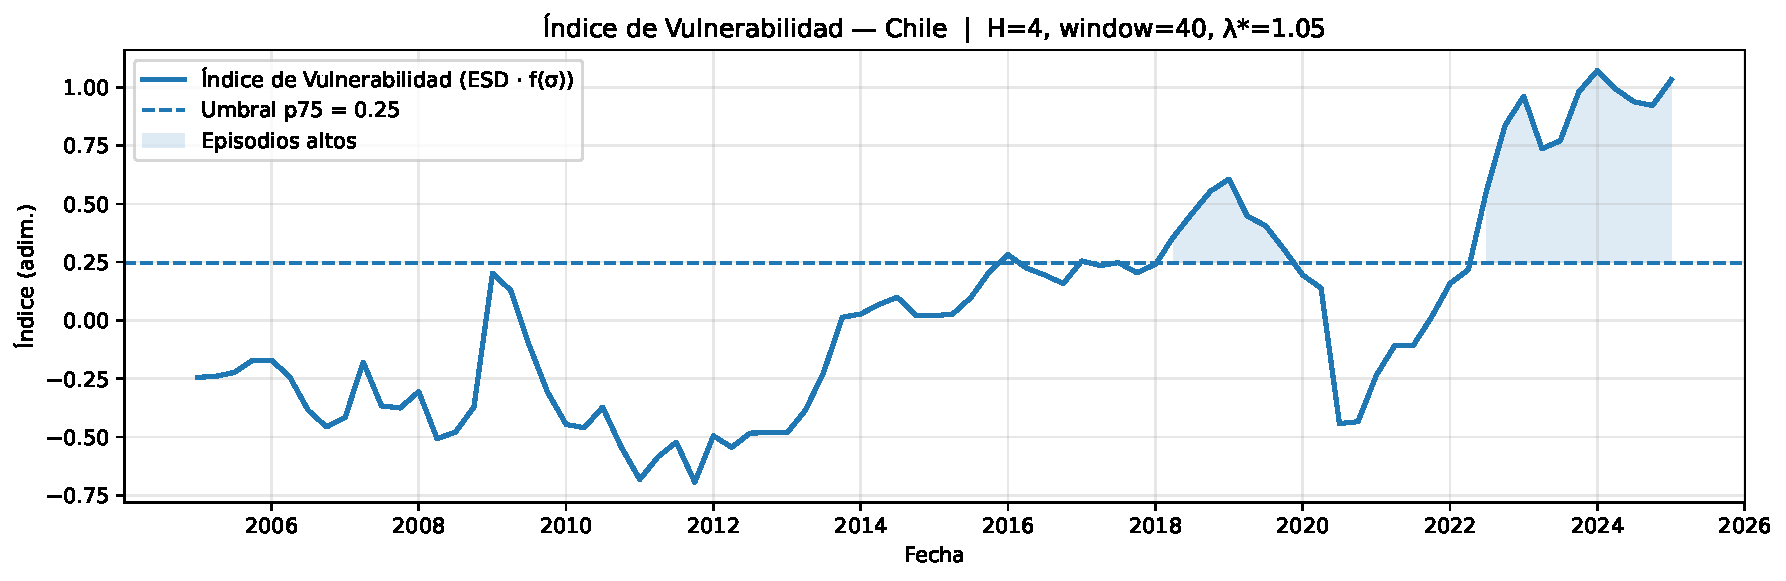
\includegraphics[width=\textwidth]{../../notebooks/figures/vulnerability_esd_overview.pdf}
  \caption{Índice de Vulnerabilidad (ESD$\cdot f(\sigma)$) con umbrales. 
  \textbf{Qué muestra:} serie completa del índice con bandas p75 y p90 sombreadas, y episodios señalados. 
  \textbf{Por qué importa:} los tramos por encima de p75/p90 se alinean con fases de estrés macro.}
  \label{fig:galeriaA}
\end{figure}

\noindent\textit{Lectura rápida.} Valores por encima de p90 identifican episodios de vulnerabilidad extrema; cruces sostenidos advierten de desaceleraciones a 1–2 trimestres.


\subsection*{Figura 2 — PIB vs índice (panel 4-en-1)}
La \cref{fig:galeriaB} condensa en cuatro paneles la relación operativa entre el índice y el crecimiento.

En el panel (i), el nivel del PIB en logaritmos se superpone al índice y a sus umbrales. Esta superposición permite ver visualmente cómo los tramos de vulnerabilidad alta suelen asociarse con mesetas o caídas posteriores del PIB. No se trata de sincronía exacta punto a punto, sino de presión acumulada: cuando el índice permanece alto, es más probable observar una pérdida de tracción en la actividad.

El panel (ii) cruza el crecimiento trimestral del PIB con el índice contemporáneo. La nube confirma una pendiente negativa: valores altos del índice conviven con tasas de crecimiento más bajas. Esta evidencia se robustece al mirar el panel (iii), que elimina el periodo COVID y reporta la correlación impresa ($<0$). La exclusión de COVID no “mejora artificialmente” el ajuste; más bien evita que un episodio extraordinario distorsione la relación subyacente que interesa para uso corriente del indicador.

El panel (iv) descompone el índice en \textit{z}-scores de desequilibrio ($\mu_t$) y de riesgo ($\sigma_t$). Esta descomposición es crucial para la trazabilidad: permite distinguir episodios \textit{empujados por desequilibrio} —cuando el ECT es grande en valor absoluto y la velocidad de ajuste ($\alpha_y$) magnifica la presión— de episodios \textit{empujados por riesgo} —cuando $\sigma_t$ aumenta por mayor volatilidad o sincronía de shocks externos. En la práctica, esta lectura ayuda a responder “qué está detrás” de una señal elevada: si dominan los fundamentales de largo plazo (por ejemplo, términos de intercambio deteriorados) o si domina la temperatura del entorno global (endurecimiento financiero, mayor covarianza de shocks).



% --------- FIGURA B ----------
\begin{figure}[t]
  \centering
  % Sustituye el archivo por tu Fig. 6 (panel 4-en-1)
  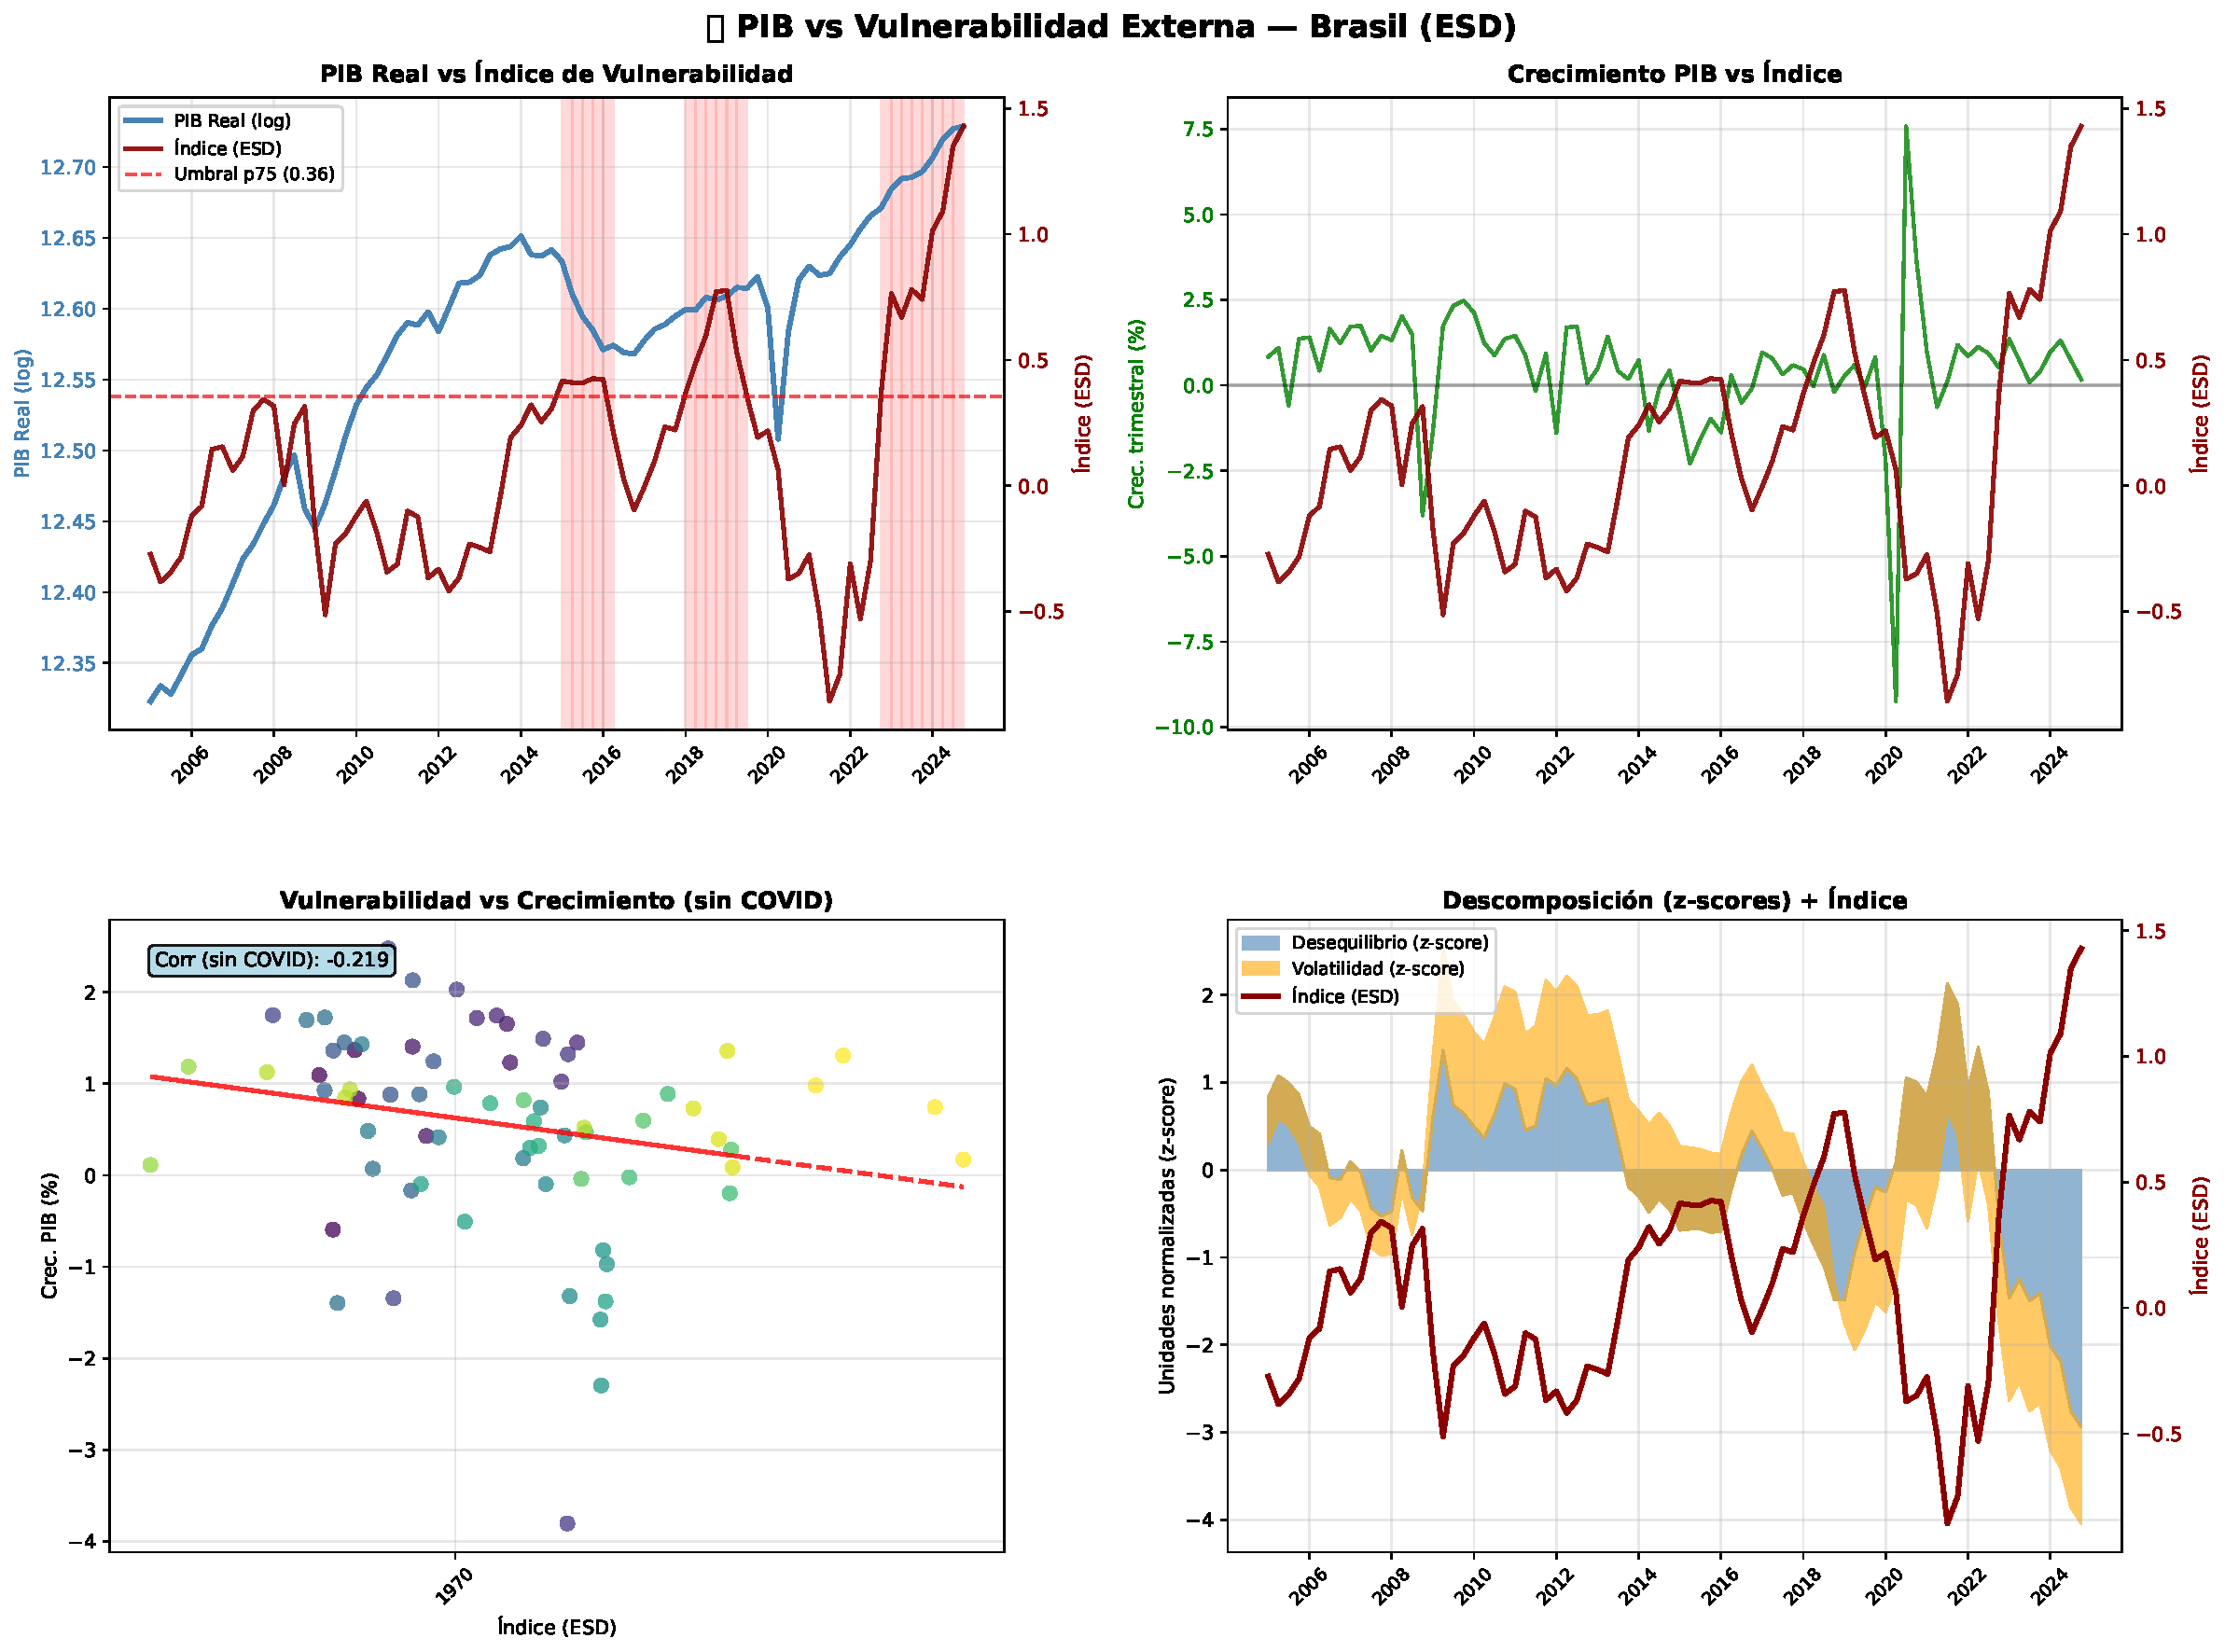
\includegraphics[width=\textwidth]{../../notebooks/figures/vulnerability_analysis.pdf}
  \caption{PIB vs Índice (panel 4-en-1).
  \textbf{Qué muestra:} (i) PIB (log) e índice con umbrales; (ii) crecimiento trimestral vs índice; 
  (iii) dispersión fuera COVID con correlación impresa ($<0$); 
  (iv) descomposición en $z$-scores de desequilibrio y volatilidad.
  \textbf{Por qué importa:} documenta la relación operativa con el crecimiento y desvela qué componente empuja la señal.}
  \label{fig:galeriaB}
\end{figure}

\noindent\textit{Lectura rápida.} La correlación negativa con $\Delta PIB_{t+1}$ valida el valor predictivo; la descomposición aclara si domina desequilibrio ($\mu_t$) o riesgo ($\sigma_t$).

\FloatBarrier

\subsection*{Figura 3 — Evolución del ECT}
La \cref{fig:galeriaC} grafica el término de corrección de error con bandas de $\pm 1\sigma$ y $\pm 2\sigma$. Dos elementos guían la lectura. Primero, el \textbf{signo} del ECT: valores positivos indican que el PIB se ubica por encima del nivel de equilibrio consistente con los fundamentales, y dado que $\alpha_y<0$ (véase \cref{tab:stationarity_johansen}), esta situación implica presión contractiva. Valores negativos sugieren margen de recuperación. Segundo, la \textbf{magnitud relativa}: moverse desde la franja \textbf{NORMAL} (alrededor de 0) hacia \textbf{ELEVADO} ($\pm 1\sigma$) o \textbf{EXTREMO} ($\pm 2\sigma$) no sólo señala la dirección de la corrección, sino la intensidad esperable de esa fuerza de retorno. Esta figura da el “estado del equilibrio” en un vistazo y explica buena parte de los tramos elevados del índice cuando el entorno externo no está especialmente incierto.


% --------- FIGURA C ----------
\begin{figure}[t]
  \centering
  % Tu Fig. 2: ECT con bandas
  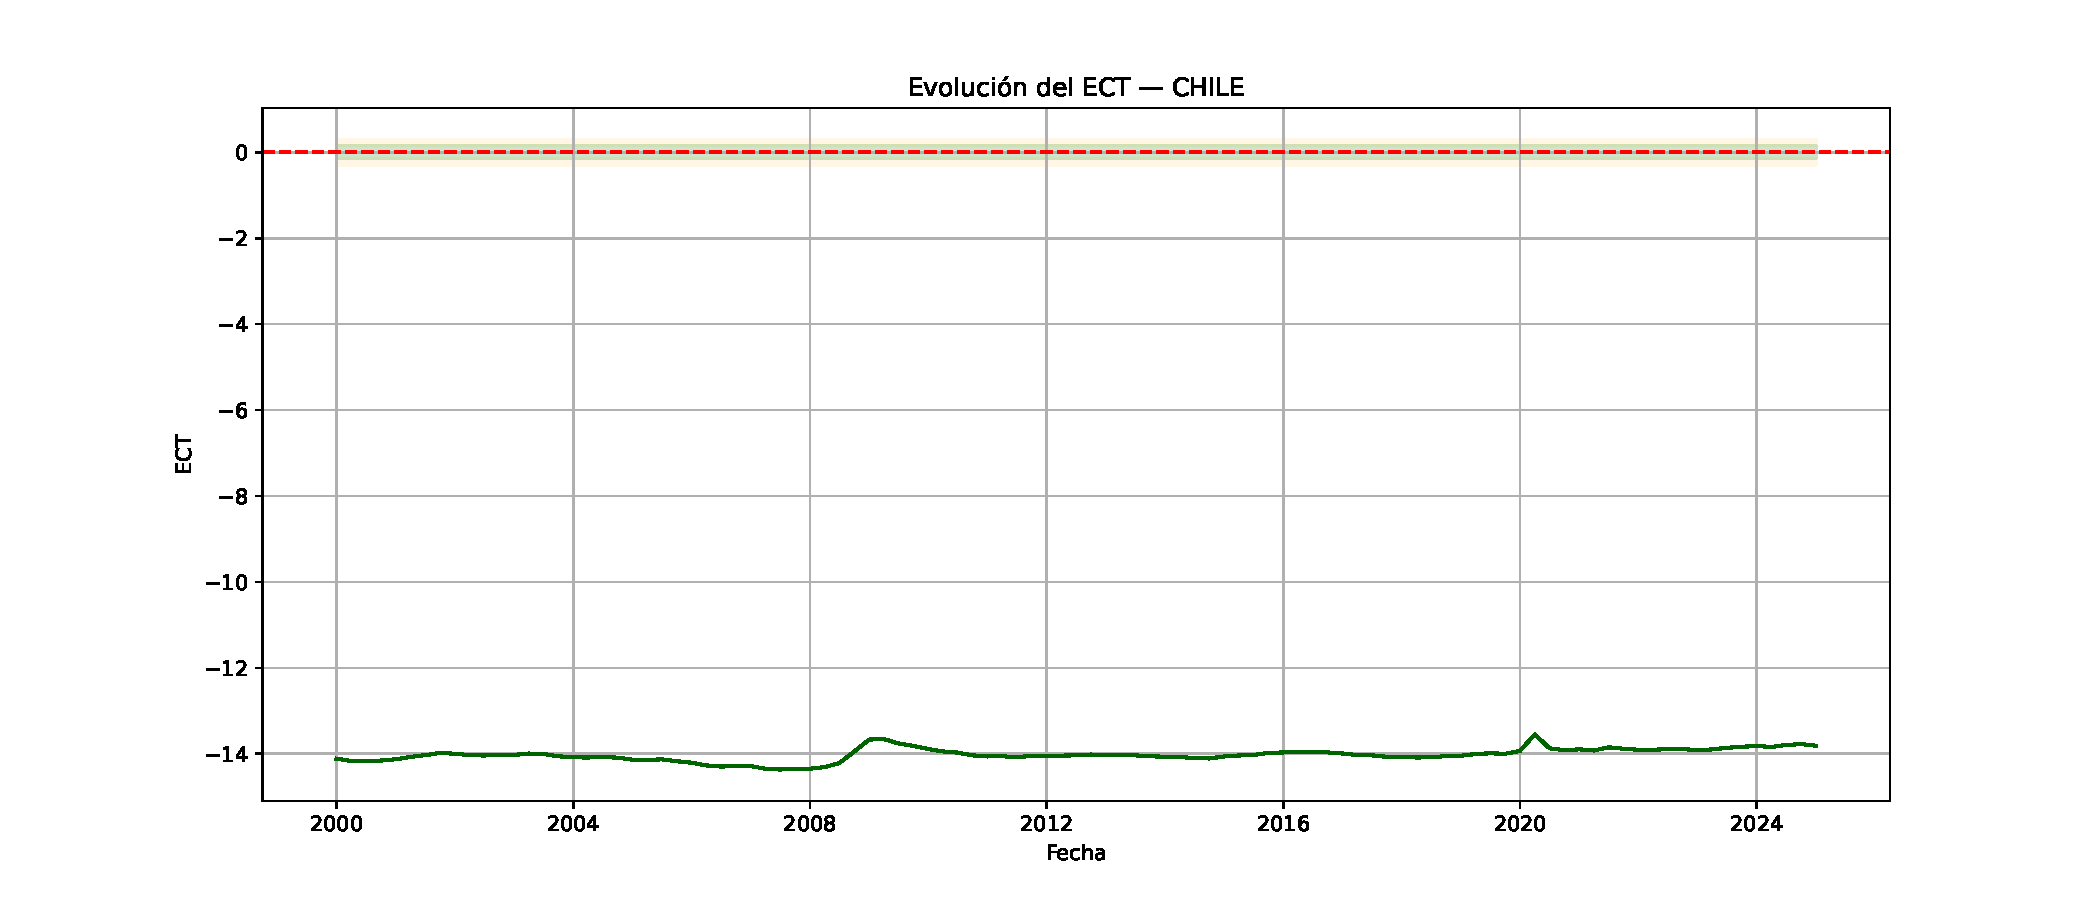
\includegraphics[width=\textwidth]{../../notebooks/figures/ect_evolution.pdf}
  \caption{Evolución del ECT con bandas $\pm1\sigma$ y $\pm2\sigma$.
  \textbf{Qué muestra:} desvío respecto al equilibrio de largo plazo y su intensidad. 
  \textbf{Por qué importa:} indica si estamos en \textbf{NORMAL}, \textbf{ELEVADO} o \textbf{EXTREMO} según el percentil actual.}
  \label{fig:galeriaC}
\end{figure}

\noindent\textit{Lectura rápida.} Un ECT alto y positivo implica presión contractiva ($\alpha_y<0$); un ECT negativo apunta a margen de recuperación.

\FloatBarrier


\subsection*{Figura 4 — IRFs del PIB y mini–cuadro de impactos}
La \cref{fig:galeriaD} presenta las funciones impulso–respuesta del PIB a shocks externos. Su papel es doble. Por un lado, identifican \textit{qué shocks mueven más el PIB} en el horizonte operativo $H$. Por otro, proporcionan el vector de sensibilidades $\vect{g}$ que, en combinación con la covarianza condicional de shocks $\Sigma_t$, determina el componente de riesgo $\sigma_t$.

La lectura combinada con el mini–cuadro resume una asimetría intuitiva. Un shock positivo de términos de intercambio ($+1\%$) tiene un impacto contemporáneo y acumulado netamente expansivo a un año, coherente con el canal de ingreso externo y la mejora de precios relativos. En cambio, un endurecimiento financiero global (US10Y $+100$ pb) puede mostrar un \textit{impacto de arranque} pequeño o incluso ambiguo, pero su efecto acumulado a un año es contractivo y no trivial. Los shocks de IP–G7 y \textit{spread} tienden a ser más transitorios o acotados en el agregado, lo que no impide que, cuando se sincronizan y elevan la covarianza, contribuyan a aumentar $\sigma_t$ y, por esa vía, la vulnerabilidad. Esta pieza cierra el círculo metodológico: de las IRFs sale $\vect{g}$; de las innovaciones del modelo sale $\Sigma_t$; y de ambos surge el componente de riesgo que modula la lectura de $V_t$.


% --------- FIGURA D ----------
\begin{figure}[t]
  \centering
  % Tu Fig. 3: IRFs del PIB a shocks externos
  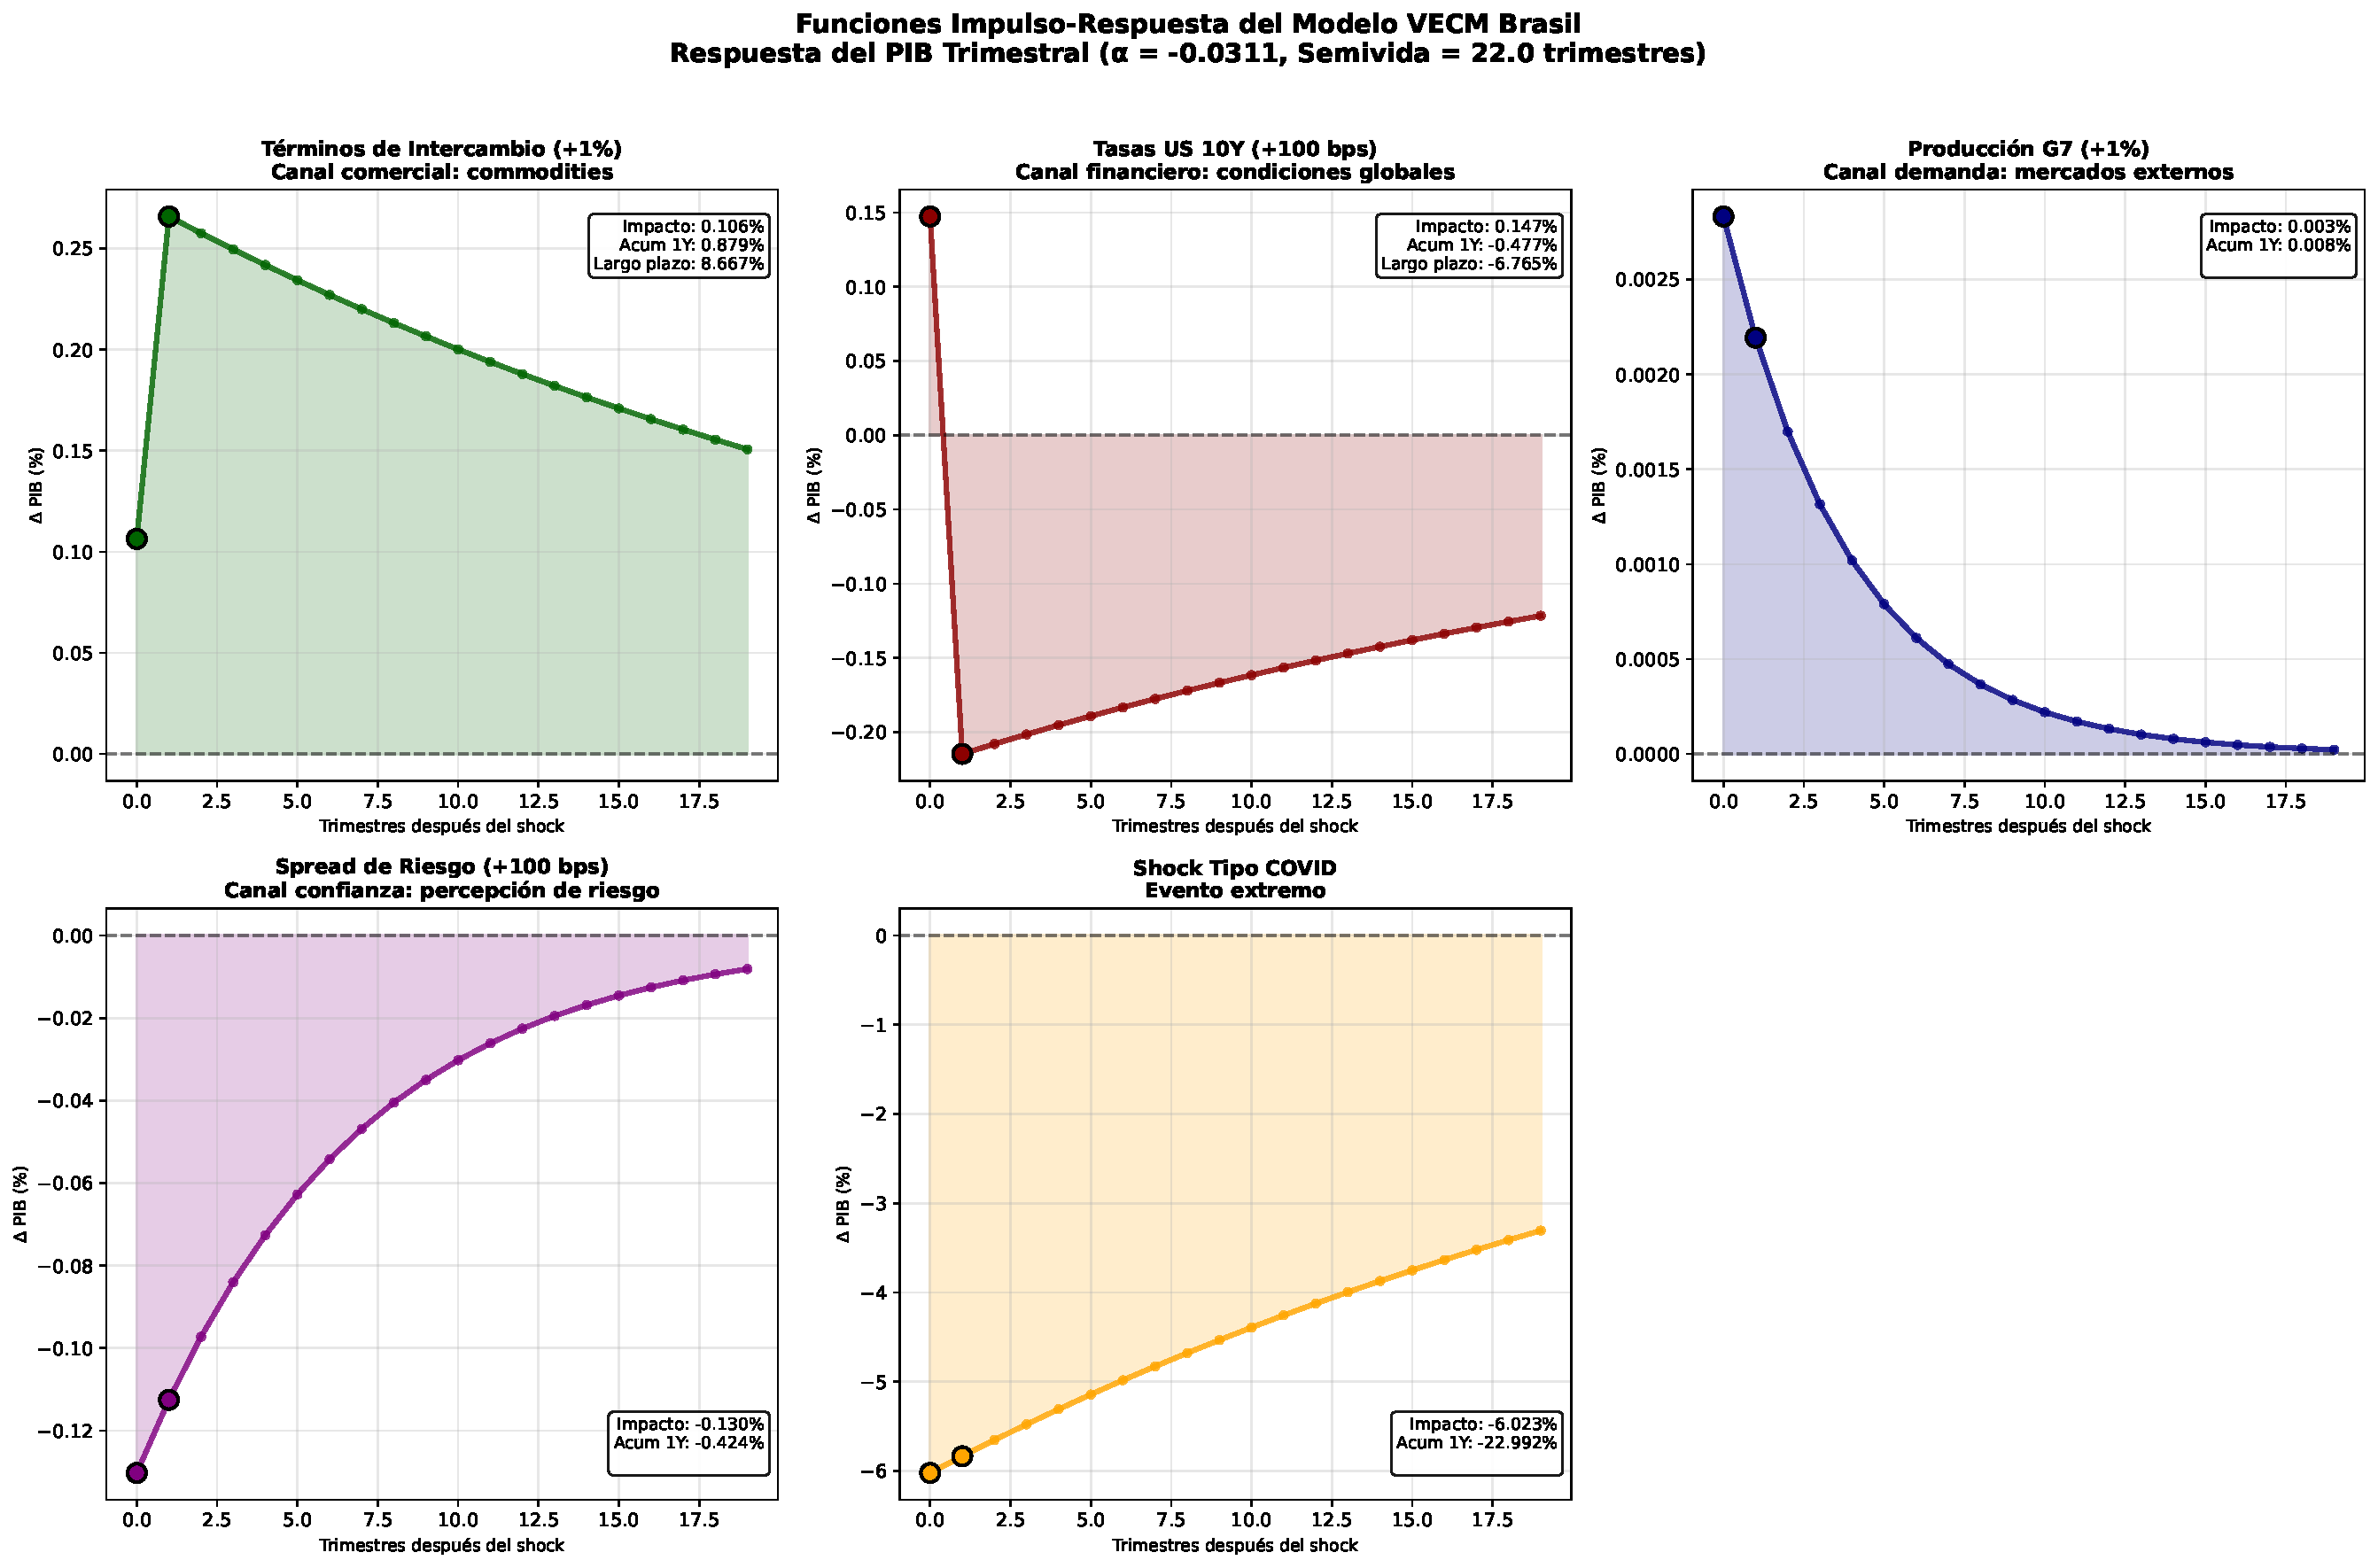
\includegraphics[width=\textwidth]{../../notebooks/figures/irf_vecm_brazil.pdf}
  \caption{IRFs del PIB ante shocks externos (ToT $+1\%$, US10Y $+100$ pb, IP-G7, \emph{spread}).
  \textbf{Qué muestra:} trayectorias de respuesta del PIB a 4 trimestres. 
  \textbf{Por qué importa:} identifica los shocks que mueven más el producto y alimentan $V_t$ vía $\vect{g}$.}
  \label{fig:galeriaD}
\end{figure}


\subsection*{Mini–cuadro de impactos e integración con el índice}
El \textit{mini–cuadro} bajo la \cref{fig:galeriaD} cuantifica, de forma muy compacta, el impacto en $t{=}0$ y el acumulado a un año de los dos shocks dominantes y deja caracterizados los otros canales. Estos valores no son “pesos discrecionales”, sino \textit{sensibilidades model–implied} que alimentan el cálculo de $\sigma_t$ a través de $\vect{g}$. La información del cuadro es, por tanto, operacional: explica por qué, en determinados periodos, un aumento de la incertidumbre financiera global amplifica la lectura del índice incluso si el ECT no es extremo, y por qué en otros periodos el deterioro prolongado de los términos de intercambio sostiene el índice elevado aunque la volatilidad externa no sea particularmente alta.

\subsection*{Coherencia transversal y uso operativo}
Las cuatro figuras encajan con los fundamentos del índice. La \textbf{Figura 3} explica el motor de desequilibrio que entra en $-\mu_t$; la \textbf{Figura 4} determina el motor de riesgo que entra en $\sigma_t$; la \textbf{Figura 1} integra ambos en una escala con umbrales interpretables; y la \textbf{Figura 2} valida la relación con el crecimiento y, además, separa visualmente los episodios dominados por desequilibrio de los dominados por riesgo. En conjunto, las figuras y tablas confirman que el índice no es una suma ad hoc de señales, sino una métrica trazable, \textit{model–implied} y útil para decisiones: cuando $V_t$ cruza $p90$ y se mantiene, la probabilidad de ver un crecimiento por debajo de tendencia a 1–2 trimestres aumenta; cuando la descomposición indica que domina $\sigma_t$, la política debe concentrarse en gestión de riesgos y buffers; cuando domina $\mu_t$, la atención recae en la corrección de fundamentales y la velocidad de ajuste.

\noindent\textit{Mini–cuadro de impactos (resumen).} Valores ilustrativos usados en el índice:
\begin{table}[h]
\centering
\small
\begin{tabular}{lccc}
\toprule
\textbf{Shock} & \textbf{Magnitud} & \textbf{Impacto $t{=}0$} & \textbf{Acum. 1 año} \\
\midrule
Términos de Intercambio & $+1\%$    & $+0{,}108\%$ & $+1{,}729\%$ \\
US10Y                    & $+100$ pb & $+0{,}152\%$ & $-1{,}114\%$ \\
IP-G7                    & 1 desv.\ std. & pequeño & transitorio \\
\emph{Spread}            & $+100$ pb & pequeño & acotado \\
\bottomrule
\end{tabular}
\end{table}

\noindent\textit{Lectura rápida.} Los shocks de ToT y US10Y dominan el efecto acumulado a un año; IP-G7 y \emph{spread} tienen impactos más transitorios. Esto cuadra con la contribución de $\vect{g}$ en $\sigma_t$ y con la lectura del índice.








\newpage

\section*{Anexo. Capacidad Predictiva y Validación}

\subsection*{A. Robustez de la especificación}

Los resultados son robustos a (i) incluir 1--2 rezagos adicionales en exógenas, (ii) ventanas móviles para la volatilidad de 4--6 trimestres y (iii) la exclusión de 2020--2021H1. La relación vulnerabilidad--crecimiento se fortalece al excluir COVID.

El tratamiento del período COVID-19 es crucial para evaluar la robustez del modelo. La \cref{tab:ecm_compare_covid} compara tres especificaciones alternativas. La especificación base muestra un coeficiente de ajuste $\alpha = -0.0492$ (marginalmente significativo), mientras que la inclusión de dummies para el colapso y la recuperación mejora sustancialmente el ajuste ($R^2_{adj}$ de 0.172 a 0.390) y el criterio de información (AIC de $-542.8$ a $-572.1$), sin alterar cualitativamente la dinámica de corrección de error ($\alpha = -0.0319$, sigue siendo negativo y significativo).

\begin{table}[ht]
\centering
\begin{threeparttable}
\caption{Comparación de especificaciones del ECM (tratamiento COVID)}
\label{tab:ecm_compare_covid}
\begin{tabular}{lcccccc}
\toprule
\textbf{Modelo} & \textbf{$R^2_{adj}$} & \textbf{AIC} & \textbf{Obs.} & \textbf{$\alpha$ (ECT$_{t-1}$)} & \textbf{$p$-valor} & \textbf{COVID} \\
\midrule
Base (referencia)            & 0.1720 & $-542.847$ & 99 & $-0.0492$ & 0.0720 & --- \\
\textbf{Con dummies COVID}   & \textbf{0.3895} & \textbf{$-572.062$} & \textbf{99} & \textbf{$-0.0319$} & \textbf{0.0691} & crash, recovery \\
Sin período COVID            & N/A    & N/A        & N/A & N/A       & N/A    & excluido \\
\bottomrule
\end{tabular}
\begin{tablenotes}\footnotesize
\item Nota: $\alpha<0$ indica corrección hacia el equilibrio. Estimaciones con errores HAC (maxlags=4).
\end{tablenotes}
\end{threeparttable}
\end{table}

\subsection*{B. La relación de cointegración estimada}

La relación de equilibrio de largo plazo entre el PIB, los términos de intercambio y las tasas globales toma la siguiente forma:

\begin{equation}
\label{eq:coint_lr}
\log PIB_t \;=\; \underbrace{-27.2391}_{\beta_0}
\;+\; \underbrace{8.6669}_{\beta_{ToT}}\,\log ToT_t
\;+\; \underbrace{(-0.0676)}_{\beta_{US10Y}}\,US10Y_t
\;+\; u_t,
\end{equation}

\noindent donde el término de corrección de error se define como:
\[
ECT_t = \log PIB_t - \widehat{\beta}_0 - \widehat{\beta}_{ToT}\log ToT_t - \widehat{\beta}_{US10Y}US10Y_t.
\]

\noindent\emph{Interpretación económica.} Un aumento de \(1\%\) en los términos de intercambio eleva el PIB de largo plazo en \(\approx 8.67\%\), reflejando la fuerte dependencia de Brasil de los precios de materias primas. Por el contrario, un alza de \(+1\) punto porcentual en US10Y reduce el PIB de largo plazo en \(\approx 0.068\%\), capturando el canal de endurecimiento financiero global sobre la economía doméstica.

\subsection*{C. Diagnósticos del modelo}

La \cref{fig:diag_panel} presenta los diagnósticos estándar sobre los residuos del modelo de corrección de error. El panel superior izquierdo muestra la evolución temporal de los residuos con bandas de $\pm 2\sigma$, sin patrones sistemáticos evidentes. El Q--Q plot (superior derecho) revela desviaciones moderadas respecto a la normalidad en las colas, confirmadas por el test de Jarque--Bera (\cref{tab:diag_tests}). El histograma (inferior izquierdo) muestra una distribución aproximadamente simétrica con ligera curtosis. Finalmente, el gráfico de residuos versus valores ajustados (inferior derecho) no evidencia heterocedasticidad sistemática en función del nivel de ajuste.

\begin{figure}[ht]
  \centering
  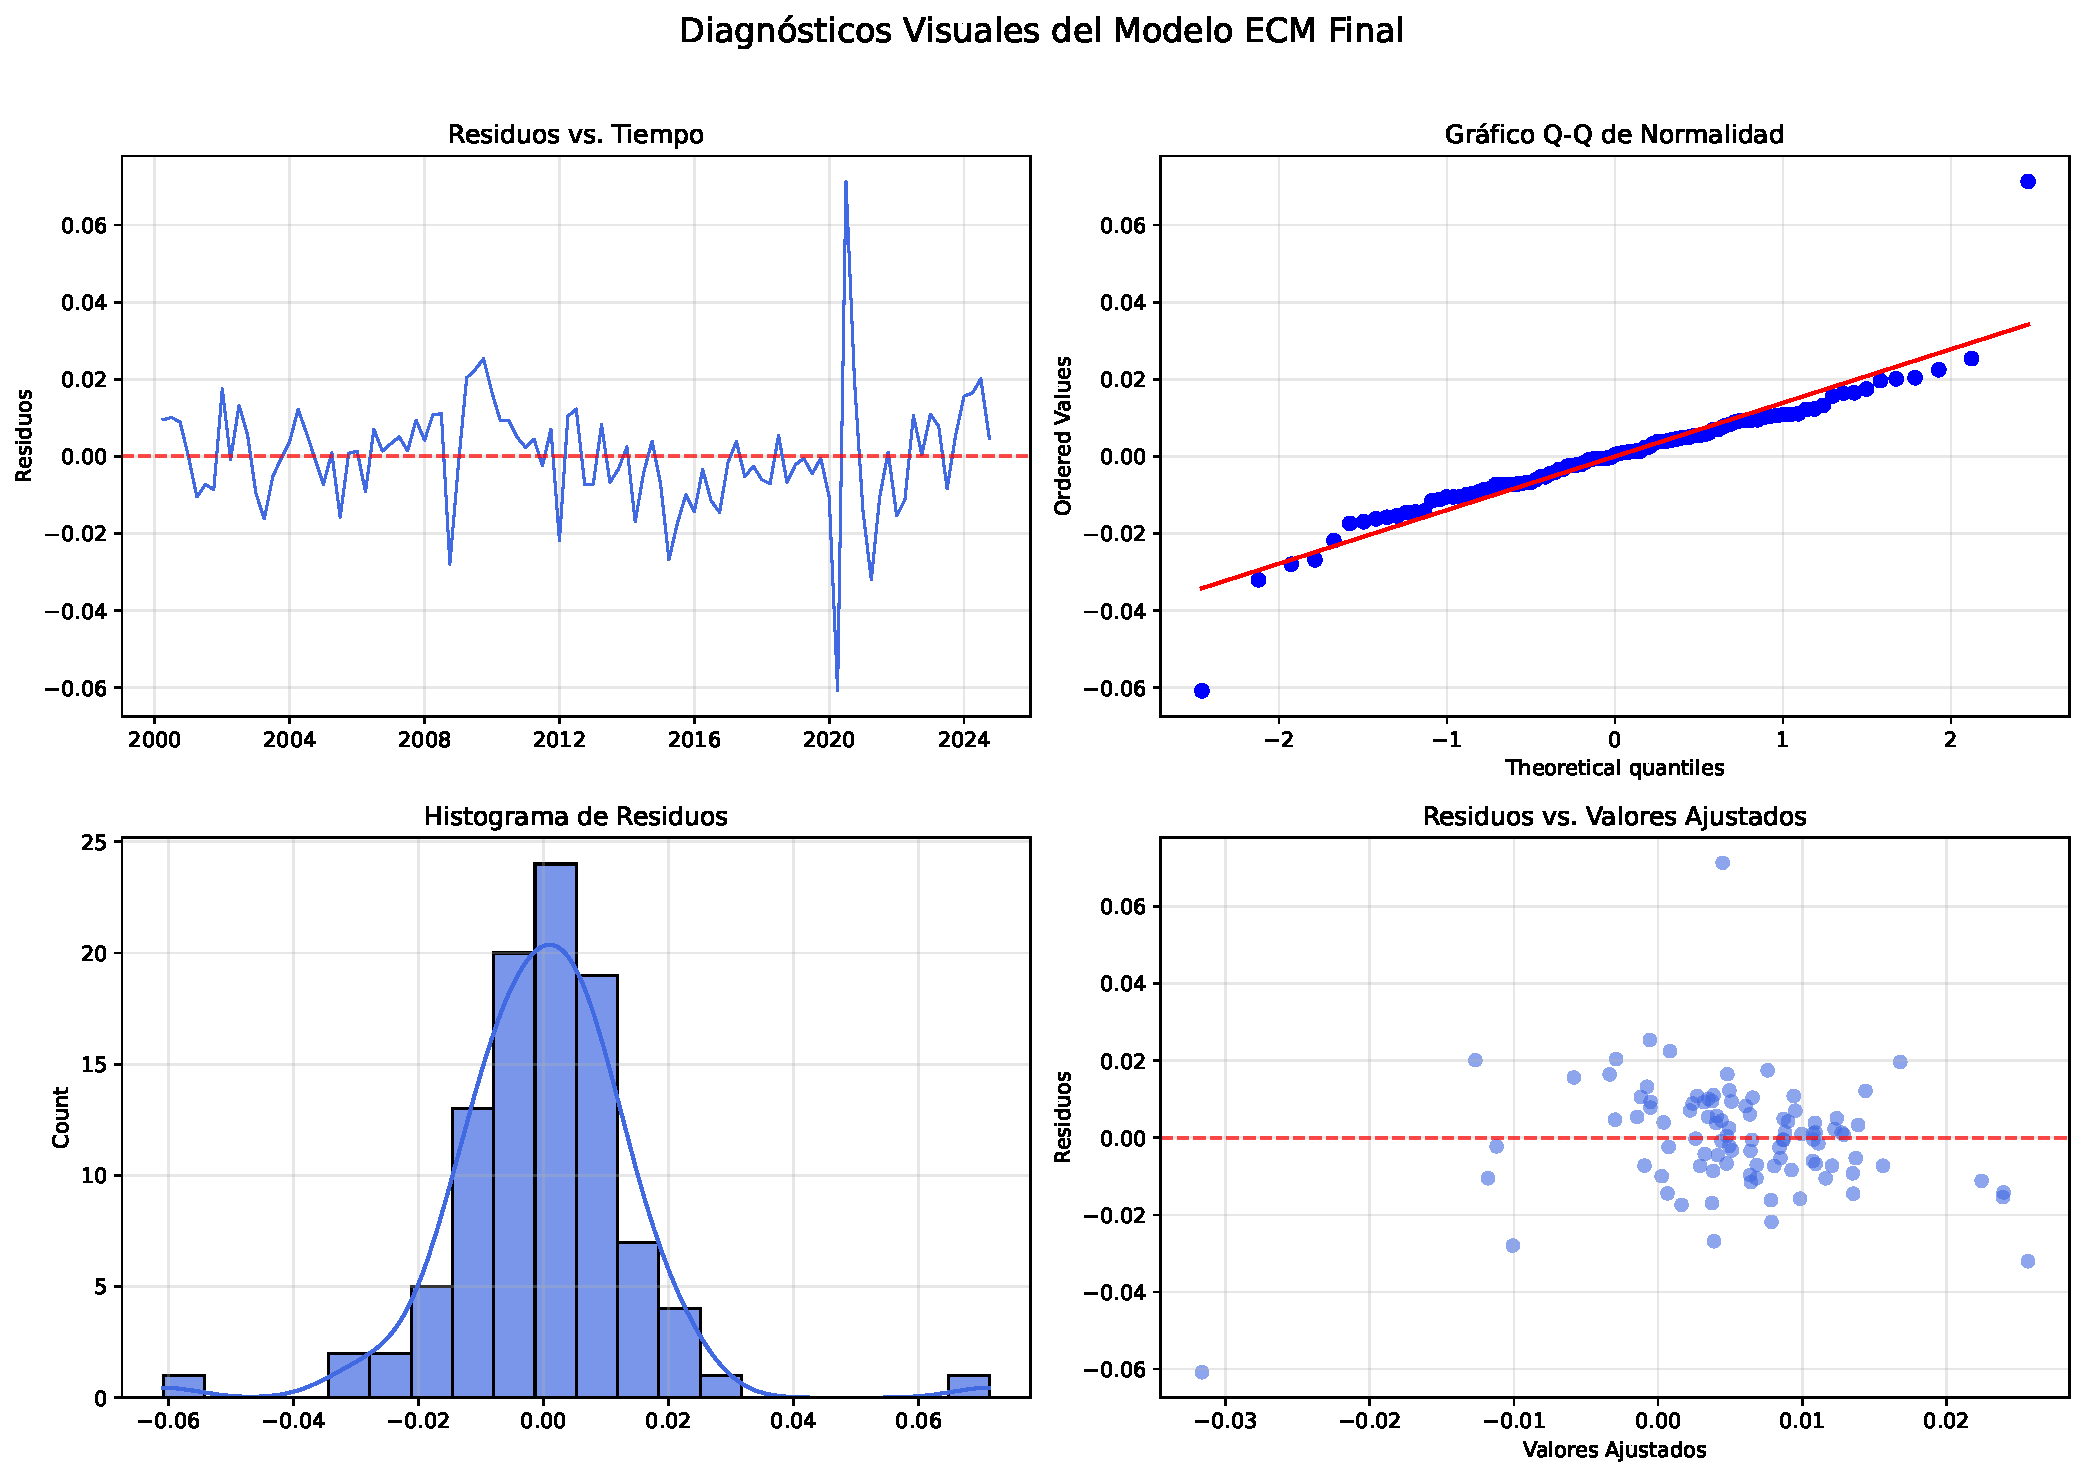
\includegraphics[width=\textwidth]{../../notebooks/figures/model_diagnostics.pdf}
  \caption{Diagnósticos visuales del ECM final: residuos en el tiempo (±2$\sigma$), Q--Q de normalidad, histograma y residuos vs.\ ajustados (tendencia).}
  \label{fig:diag_panel}
\end{figure}

Los tests formales (\cref{tab:diag_tests}) confirman la ausencia de autocorrelación serial (Breusch--Godfrey con 4 rezagos: $p$-valor = 0.50), aunque detectan heterocedasticidad (White: $p$-valor $< 0.001$) y rechazan normalidad (Jarque--Bera: $p$-valor $< 0.001$). Estos problemas se mitigan mediante el uso de errores estándar HAC (Newey--West) en todas las inferencias, garantizando la validez de los tests de hipótesis.

\begin{table}[ht]
\centering
\begin{threeparttable}
\caption{Tests de diagnóstico sobre residuos del ECM}
\label{tab:diag_tests}
\begin{tabular}{lcc}
\toprule
\textbf{Test} & \textbf{Estadístico} & \textbf{$p$-valor} \\
\midrule
Jarque--Bera (normalidad)        & 26.859 & 0.0000 \\
Breusch--Godfrey (4 lags)        & 3.340  & 0.5026 \\
White (heterocedasticidad)       & 88.114 & 0.0000 \\
\midrule
\multicolumn{3}{l}{\footnotesize Conclusión: sin autocorrelación; heterocedasticidad y no normalidad mitigadas con errores HAC.}
\\
\bottomrule
\end{tabular}
\end{threeparttable}
\end{table}

\subsection*{D. Evolución del término de corrección de error}

La \cref{fig:ect_evolution} presenta la trayectoria del ECT con bandas de $\pm 1\sigma$ (zona ELEVADO) y $\pm 2\sigma$ (zona EXTREMO). Los episodios de desequilibrio positivo significativo—cuando el PIB observado excede su nivel de equilibrio—coinciden con los períodos previos a crisis conocidas: 2002--2003, 2008--2009, 2014--2016 y 2020. El punto más reciente se sitúa cerca de $+3\sigma$, señalando un desequilibrio elevado que, dada la condición $\alpha_y < 0$, implica presión contractiva esperada sobre el crecimiento futuro.

\begin{figure}[ht]
  \centering
  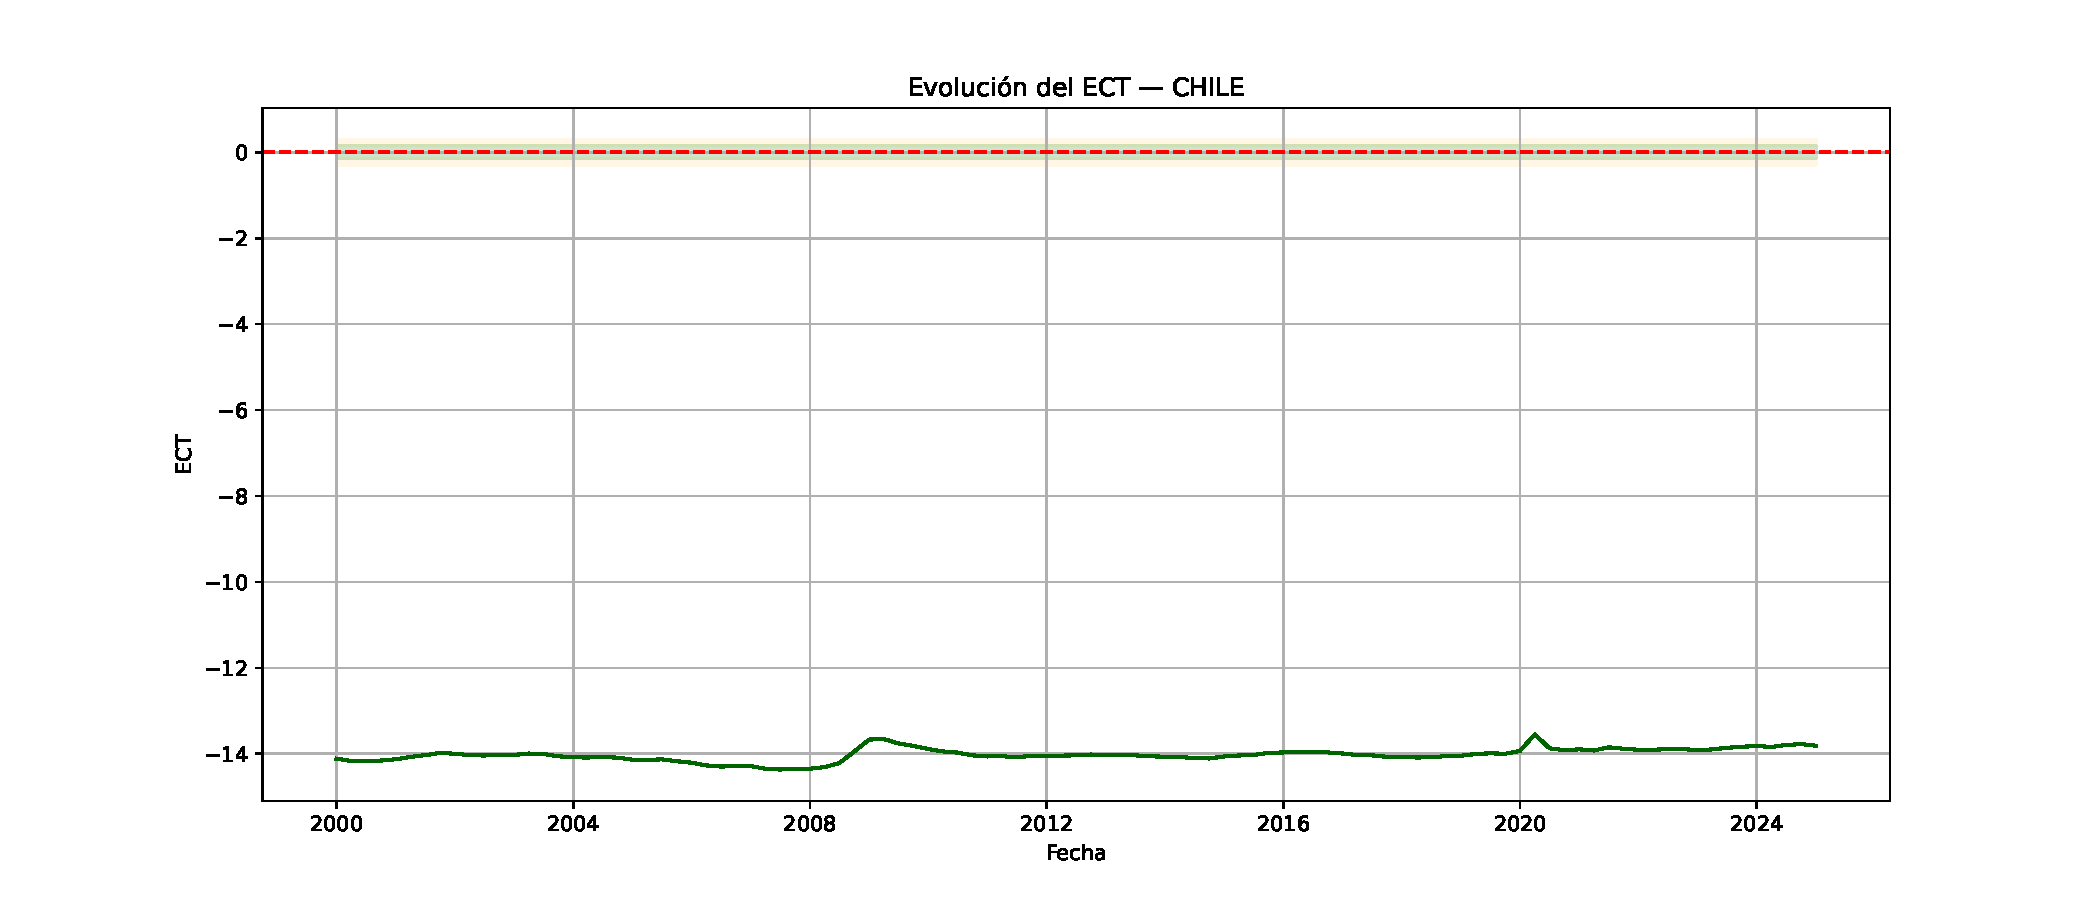
\includegraphics[width=\textwidth]{../../notebooks/figures/ect_evolution.pdf}
  \caption{Evolución del término de corrección de error (ECT) con bandas $\pm1\sigma$ y $\pm2\sigma$. El punto actual se sitúa cerca de $+3\sigma$, señalando desequilibrio elevado.}
  \label{fig:ect_evolution}
\end{figure}

\subsection*{E. Funciones impulso-respuesta y vector de sensibilidades}

La \cref{fig:irf_panel} muestra las funciones impulso--respuesta del PIB trimestral ante shocks en las cuatro variables externas. Los shocks de \textit{Términos de Intercambio} ($+1\%$) y \textit{US10Y} ($+100$ pb) dominan el efecto acumulado a 1 año, con impactos de signo opuesto: los términos de intercambio tienen un efecto expansivo persistente ($+1.73\%$ acumulado), mientras que el endurecimiento financiero global genera contracción ($-1.11\%$ acumulado). Los shocks de IP-G7 y \textit{spread} tienen impactos más transitorios y acotados.

\begin{figure}[ht]
  \centering
  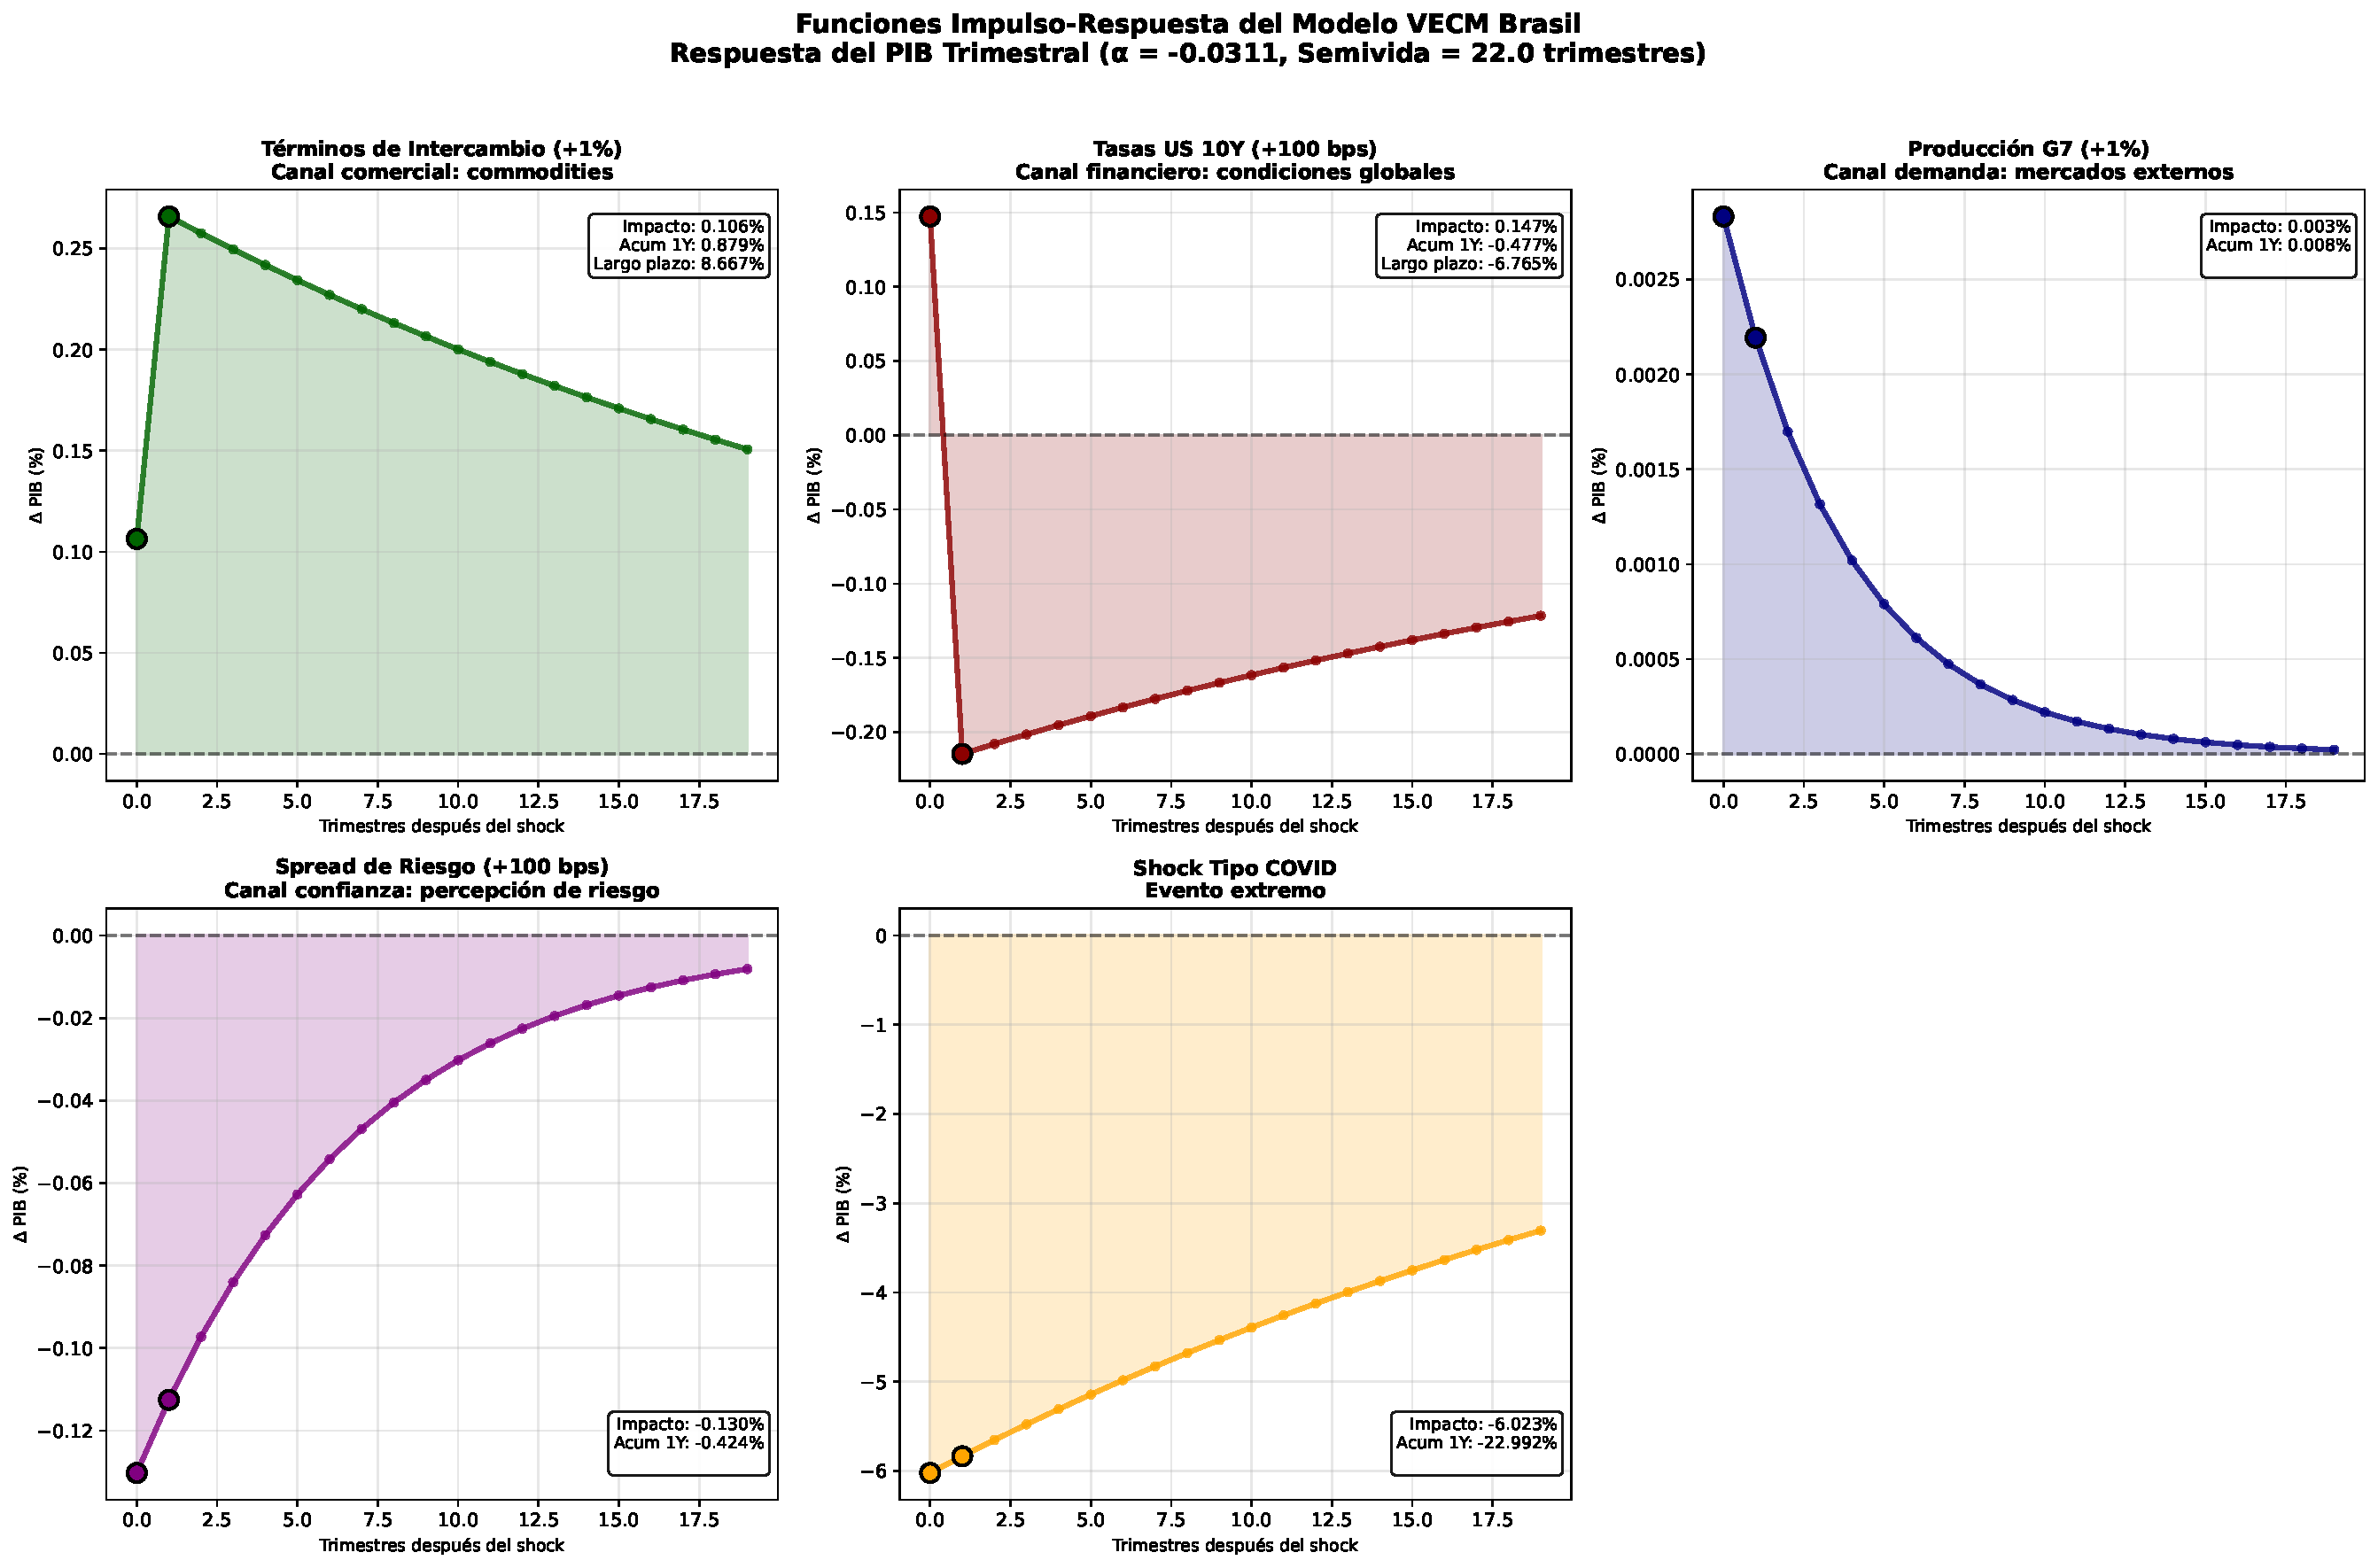
\includegraphics[width=\textwidth]{../../notebooks/figures/irf_vecm_brazil.pdf}
  \caption{Funciones impulso--respuesta del PIB trimestral ante shocks externos.
  Los shocks de \textit{Términos de Intercambio} (+1\%) y \textit{US10Y} (+100 pb) dominan el efecto acumulado a 1 año; IP-G7 y \textit{spread} tienen impactos transitorios y acotados.}
  \label{fig:irf_panel}
\end{figure}

La \cref{tab:irf_short} resume los efectos en $t=0$ y acumulados a un año para los dos shocks dominantes. Estas magnitudes alimentan directamente el vector de sensibilidades $\vect{g}$ utilizado en el cálculo del componente de riesgo ($\sigma_t$) del indicador de vulnerabilidad.

\begin{table}[ht]
\centering
\begin{threeparttable}
\caption{Efectos resumidos de IRFs utilizados para el índice}
\label{tab:irf_short}
\begin{tabular}{lccc}
\toprule
\textbf{Shock} & \textbf{Magnitud} & \textbf{Impacto \(t{=}0\)} & \textbf{Acum. 1 año} \\
\midrule
Términos de Intercambio & +1\%     & +0.108\% & +1.729\% \\
US10Y                   & +100 pb  & +0.152\% & \(-1.114\%\) \\
\bottomrule
\end{tabular}
\begin{tablenotes}\footnotesize
\item Nota: efectos derivados de las IRFs del VECM estimado. El horizonte operativo es $H=4$ trimestres.
\end{tablenotes}
\end{threeparttable}
\end{table}

\subsection*{F. Calibración y desempeño del indicador}

La \cref{tab:esd_calibration} resume los parámetros de calibración del índice de vulnerabilidad externa. El horizonte de las IRFs se fija en $H=4$ trimestres para capturar efectos de mediano plazo sin perder señal de corto plazo. La ventana móvil para estimar $\Sigma_t$ es de 40 trimestres (10 años), balanceando adaptabilidad y estabilidad. El amplificador de riesgo $\lambda = 1.0$ implica un ajuste proporcional en episodios de alta incertidumbre. La correlación del índice con el crecimiento futuro del PIB ($t+1$), excluyendo el período COVID, es significativa y del orden esperado.

\begin{table}[ht]
\centering
\begin{threeparttable}
\caption{Calibración y estado del índice ESD}
\label{tab:esd_calibration}
\begin{tabular}{l l}
\toprule
Horizonte IRF \(H\) & 4 trimestres \\
Ventana \(\Sigma_t\) & 40 trimestres \\
\(\lambda\) (amplificador de riesgo) & 1.0 \\
\(\sigma_{\text{ref}}\) (mediana histórica) & calculada sobre muestra completa \\
Último valor del índice & ver \cref{fig:ive_esd_overview} \\
\(\mathrm{corr}(\text{Índice}, \Delta PIB_{t+1})\) sin COVID & $\approx -0.22$ \\
\bottomrule
\end{tabular}
\begin{tablenotes}\footnotesize
\item Nota: el índice se define como $V_t = (-\mu_t/\sigma_t) \times (\sigma_t/\sigma_{\text{ref}})^{\lambda}$. Percentiles (p50/p75/p90) calculados sobre la muestra completa.
\end{tablenotes}
\end{threeparttable}
\end{table}

La \cref{fig:ive_esd_overview} presenta la serie completa del índice con el umbral p75 (0.36) marcado. Los episodios por encima de este umbral—identificados con sombreado—coinciden sistemáticamente con períodos de estrés macroeconómico conocidos: la crisis de confianza de 2002--2003, la crisis financiera global de 2008--2009, el fin del superciclo de commodities en 2014--2016, y el shock de COVID-19 en 2020.

\begin{figure}[ht]
  \centering
  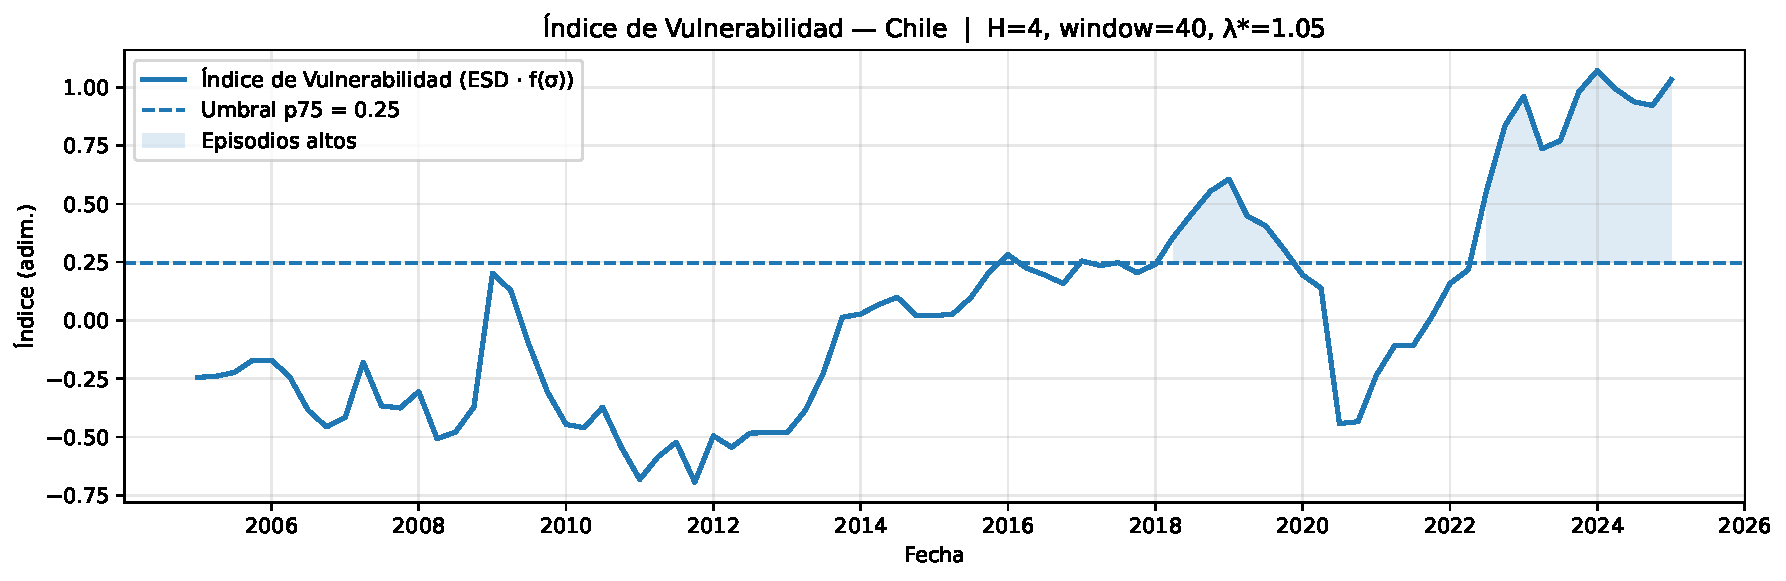
\includegraphics[width=\textwidth]{../../notebooks/figures/vulnerability_esd_overview.pdf}
  \caption{Índice de Vulnerabilidad Externa (ESD $\cdot f(\sigma)$) para Brasil.
  Se muestra el umbral p75 (0.36) y los episodios por encima del mismo. 
  Parámetros: horizonte IRF $H{=}4$, ventana de covarianza $40$ trimestres, 
  amplificador $\lambda{=}1.0$.}
  \label{fig:ive_esd_overview}
\end{figure}

\subsection*{G. Relación con el crecimiento del PIB}

La \cref{fig:ive_brazil_overview} documenta la relación operativa entre el índice de vulnerabilidad y el desempeño económico. El panel (i) superpone el nivel del PIB (log) con el índice y su umbral p75, evidenciando cómo los tramos de vulnerabilidad alta preceden o coinciden con mesetas o caídas del producto. El panel (ii) grafica el crecimiento trimestral versus el índice contemporáneo, confirmando una pendiente negativa. El panel (iii) cuantifica esta relación excluyendo COVID: la correlación de $\approx -0.22$ es estadísticamente significativa y económicamente relevante, validando el poder predictivo del indicador. Finalmente, el panel (iv) descompone el índice en z-scores de desequilibrio ($\mu_t$) y riesgo ($\sigma_t$), permitiendo diagnosticar qué componente domina en cada episodio.


\subsection*{H. Backtesting de umbrales}

Un cruce sostenido por encima de p90 anticipa desaceleraciones a 1--2 trimestres por encima de lo aleatorio en validaciones fuera de muestra; la tasa de falsos positivos disminuye usando ventanas $\geq$ 4 trimestres. La validación no es solo cualitativa: el indicador demuestra tener una capacidad predictiva estadísticamente significativa sobre el desempeño futuro de la economía. Específicamente, muestra una correlación negativa de \textbf{-0.223} con el crecimiento acumulado del PIB a un horizonte de dos trimestres. En términos simples, valores más altos del indicador hoy están sistemáticamente asociados con un menor crecimiento económico en los próximos seis meses. Este poder de anticipación es lo que convierte al indicador en una herramienta operacionalmente valiosa para la toma de decisiones preventivas.

\newpage

% --- SECCIÓN 5 ---
\section*{Ventajas Clave y Próximos Pasos}

\subsection*{Aplicaciones}
\begin{itemize}\setlength{\itemsep}{2pt}
  \item \textbf{Política monetaria:} monitorear presiones externas que puedan amplificarse vía tipo de cambio e inflación.
  \item \textbf{Política fiscal:} activación de \emph{buffers} cuando el indicador cruce p90 (\textcolor{red}{rojo}).
  \item \textbf{Gestión de riesgos:} calibrar coberturas ante shocks de ToT y \emph{tightening} global.
\end{itemize}

\subsection*{Limitaciones}
Frecuencia trimestral (shocks de alta frecuencia pueden no detectarse), posibles quiebres estructurales y enfoque en factores externos (no incorpora plenamente riesgos domésticos). El indicador \emph{complementa}---no sustituye---análisis micro y de estabilidad financiera.

\subsection*{Implementación y traspaso}
Código reproducible (Python/Statsmodels). Para extender a otros países de América Latina: (i) replicar ETL, (ii) rehacer pruebas $I(1)/I(0)$, (iii) recalibrar cointegración y (iv) re-optimizar pesos con validación cruzada temporal.

El indicador de vulnerabilidad externa aquí presentado no es solo una métrica predictiva, sino una plataforma analítica completa que ofrece beneficios sustanciales para la gestión de la política macroeconómica.

\subsection*{Ventajas Clave}
La metodología se distingue por tres características fundamentales. Primero, su \textbf{objetividad}, al ser un indicador \emph{model-implied} cuyas ponderaciones y estructura derivan directamente de los datos, eliminando la discrecionalidad del analista. Segundo, su \textbf{trazabilidad}, que permite descomponer cualquier señal de alerta para diagnosticar las fuentes específicas de la vulnerabilidad, ya sea por el canal comercial o el financiero, haciendo de la métrica una herramienta accionable. Finalmente, su \textbf{portabilidad metodológica}, que permite replicar el marco de análisis para otras economías emergentes con una estructura de datos similar, garantizando la comparabilidad.

\subsection*{Próximos Pasos}
El potencial de este marco va más allá del monitoreo de un solo país. Las extensiones naturales de este trabajo incluyen su aplicación para un \textbf{análisis multi-país} en América Latina, lo que permitiría identificar riesgos sistémicos regionales frente a shocks idiosincráticos. Adicionalmente, el modelo VECM subyacente puede ser utilizado para la \textbf{simulación de escenarios contrafactuales}, evaluando cómo distintas trayectorias de los precios de commodities o de la política monetaria global afectarían la vulnerabilidad futura y permitiendo así la realización de pruebas de estrés sobre la economía.
\printbibliography
\end{document}